\documentclass[12pt]{book}

% Package includes
\usepackage[Glenn]{fncychap}
\usepackage[margin=2cm]{geometry}
\usepackage[english]{babel} % For English language support
\usepackage{subcaption} % Add this line to include the subcaption package
\pagenumbering{arabic}
\usepackage{titling}
\usepackage{interval}
\usepackage{csquotes}
\usepackage{tabularx}
\usepackage{comment}
\usepackage{natbib}
\usepackage{amssymb}
\usepackage{graphicx}
\usepackage{tikz}
\usepackage[ruled,vlined]{algorithm2e}
\usepackage{algorithmicx}
\usepackage{algpseudocode}
\usepackage{booktabs}
%\usepackage[framed,numbered,autolinebreaks,useliterate]{mcode}
\usepackage{url,textcomp}
\usepackage{graphicx,wrapfig}
\usepackage{rotating}
\usepackage{float}
\usepackage{multirow}
\usepackage{eurosym} % For the euro symbol
\usepackage{color}
\usepackage{listings}
\definecolor{mygreen}{RGB}{28,172,0} % Color values Red, Green, Blue
\definecolor{mylilas}{RGB}{170,55,241}
\usepackage{amsmath}
\usepackage{lscape}
\usepackage{subfig}
\usepackage{colortbl}
\usepackage{parskip}
%\usepackage[dvipsnames]{xcolor}
\usepackage{fancyhdr}
\usepackage{vmargin}
\usepackage{pdfpages}

% Load hyperref and cleveref in the correct order
\usepackage{cleveref}
\usepackage{url,textcomp}

\usepackage[titletoc]{appendix}
\usepackage{titlesec}

% Section number depth settings
\setcounter{secnumdepth}{4}
\titleformat{\paragraph}
{\normalfont\normalsize\bfseries}{\theparagraph}{1em}{}
\titlespacing*{\paragraph}
{0pt}{3.25ex plus 1ex minus .2ex}{1.5ex plus .2ex}

% Customizing chapter headings
\usepackage{etoolbox}
\makeatletter
\patchcmd{\@makechapterhead}{\vspace*{50\p@}}{\vspace*{-20\p@}}{}{}
\patchcmd{\@makeschapterhead}{\vspace*{50\p@}}{\vspace*{-20\p@}}{}{}
\patchcmd{\DOTI}{\vskip 80\p@}{\vskip 40\p@}{}{}
\patchcmd{\DOTIS}{\vskip 40\p@}{\vskip 0\p@}{}{}
\makeatother

% Customizing appendix names
\renewcommand{\appendixpagename}{Anexos}
\renewcommand{\appendixtocname}{Anexos}
\renewcommand{\appendixname}{Anexo}

% Footer and header settings
\renewcommand{\footrulewidth}{0.5pt}
\renewcommand{\rmdefault}{\sfdefault}

% Bibliography settings
%\usepackage{biblatex} % Imports biblatex package
%\addbibresource{jrz.bib} % Import the bibliography file

% Graphics path
\graphicspath{{figures/}} % Folder for figures

% Title setup
\title{TFM}
\makeatletter
\let\thetitle\@title
\let\theauthor\@author
\let\thedate\@date
\makeatother

% Fancy headers and footers
\pagestyle{fancy}
\fancyhf{}
\rhead{Master in Mathematics}
\lhead{Final Master Degree}
\rfoot{\thepage}
\lfoot{University of Granada}

\begin{document}

\usetikzlibrary{arrows}

\begin{titlepage}
      \begin{center}
%%%\includegraphics[scale=1.2]{Fotos/Cap0/Logo.png}%incluir el logo
      \end{center}
      \vspace{2cm}
 %%%%%%%%%%%%%%%%%%%%%%%%%%%     
   \begin{center}
      \huge\textbf{Smart Road Pricing Strategies for Sustainable Tourism Management in Sierra Nevada National Park: Insights from a Dynamic Field Study}\\
      \end{center}
       \vspace{1 cm}
      
         \begin{center}
      \large\textbf{Trabajo Fin de Máster}\\
      \large\textbf{Curso académico 2023/2024}\\
      \large\textbf{Máster Universitario en Matemáticas}\\
      \end{center}
 %%%%%%%%%%%%%%%%%%%%%%%%%%%  
      \vspace{2 cm}
      \begin{center}
\large\textit{Trabajo realizado por: Alberto Jesús Durán López}\\
 \large\textit{Tutor: Blanca Delgado Márquez}\\
\large\textit{Co-tutor: Miguel Luis Rodríguez González}\\

\vspace{3.5 cm}
 %%%%%%%%%%%%%%%%%%%%%%%%%%%  
\large \textbf{Universidad de Granada} \\
\large \textbf{Escuela Internacional de Posgrado} \\
\end{center}
   \vspace*{\stretch{2.0}}
\end{titlepage}



\newpage
\thispagestyle{empty}
\mbox{}
\newpage

\thispagestyle{empty}

\vfill

\begin{center}
    \textsc{\huge Declaración de originalidad}\\[1cm]
\end{center}

\noindent D. \textbf{Alberto Jesús Durán López} \\\medskip

\noindent Declaro explícitamente que el trabajo presentado como Trabajo de Fin de Máster (TFM), correspondiente al curso académico 2023-2024, es original, entendido esto en el sentido de que no he utilizado para la elaboración del trabajo fuentes sin citarlas debidamente.
\medskip

\noindent En Granada a 5 de Julio de 2024.
\vspace{3cm}

\begin{center}
    Fdo: \textbf{Alberto Jesús Durán López.}
\end{center}

\vfill

\newpage
\thispagestyle{empty}
\mbox{}
\newpage



 %%%%%%%%%%%%%%%%%%%%%%%%%%%  

\tableofcontents
%\listoffigures
%por si quieres cambiar el nombre
%\renewcommand\listtablename{Índice de tablas}
%\listoftables
%\clearpage
%\mainmatter

%%%%%%%%%%%%%%%%%%%%%%%%%%%%%%%5 AGRADECIMIENTOS
%\newpage
%\chapter*{Agradecimientos}
%A todos ellos, muchas gracias.
%%%%%%%%%%%%%%%%%%%% RESUMEN 




\chapter*{Summary}


This project focuses on the Sierra Nevada National Park, specifically in the Alpujarra towns of Pampaneira, Capileira, and Bubión. The objective is to develop a dynamic pricing algorithm for parking management in the Barranco de Poqueira area. The Barranco de Poqueira annually attracts a significant number of tourists and nature enthusiasts. While this influx benefits the local economy, it also poses potential threats to the park's ecological balance. For this reason, this project proposes an alternative approach that combines machine learning techniques to develop a dynamic pricing algorithm based on a dataset of tourist visitation data in the area while preserving social responsibility, economic sustainability, and environmental preservation components. Additionally, we incorporate a behavioral component, which is based on the likelihood of future visits if a parking toll is implemented. This data is obtained through questionnaires.

First, due to the limited instances and subjective responses of survey questions, we introduce an oversampling method called KM-SMOTE, which combines K-medoids clustering with the SMOTE (Synthetic Minority Over-sampling Technique) algorithm. This method is designed to enhance the performance of our data, which is affected by noise and high dimensionality. We analyze and clean the data and compare the algorithm to other clustering-based algorithms. With this model, we predict the likelihood of returning to the Barranco de Poqueira after the implementation of a toll in a parking lot. Second, we enrich our data with this new variable to create a dynamic pricing model. The objective is to separate the variables into four categories (environmental, social, economic, and behavioral) and assign weights to the different features using a predefined strategy. Thus, the weights assigned to each feature will be used to assign prices in a price assignment function. Finally, we create a regression model to understand the impact of each feature on the final price, allowing us to validate the pricing algorithm and adjust the weights of the variables if needed.

The goal of this project is to implement our contributions in the Alpujarra region within the Sierra Nevada National Park to dynamically assign toll prices to vehicles. This approach, accompanied by data collection over several months, allows for dynamic price assignments for new vehicles entering the area. This prepares stakeholders to manage and prevent overcrowding in the Barranco de Poqueira, ensuring sustainable tourism management and enhancing the visitor experience. The dynamic pricing algorithm aims to minimize high traffic in sensitive areas, promote the use of eco-friendly transportation, and distribute the economic benefits of tourism more evenly across the region.

\begin{comment}
    
\newpage
\chapter*{Glossary of terms}
\begin{table}[H]
\centering
\begin{tabular}{r|l}

NLP & \textit{Natural language processing} \\
LPR & \textit{License plate recognitiion} \\
WCSS & \textit{Within cluster sum of squares} \\
TP & \textit{True positives} \\
TN & \textit{True negatives} \\
FP & \textit{False positives}\\
FN & \textit{False negatives} \\
MAE & \textit{Mean absolute error} \\
MSE & \textit{Mean squared error} \\
RMSE & \textit{Root mean squared error} \\
$R^2$ & \textit{Coefficient of determination} \\
MAPE & \textit{Mean absolute percentage error} \\
SMOTE & \textit{Synthetic Minority Oversampling Technique} \\
\end{tabular}
\end{table}
\end{comment}




\chapter{Introduction}

\section{Motivation}

In recent years, machine learning has become increasingly important in various areas of society, such as education \citep{bujang2021multiclass,aburayya2023sem}, health \citep{das2023patient,garcia2020cnn}, economics \citep{kumar2022systematic,lokanan2022fraud}, and tourism \citep{kitsios2022user,bolanos2024clustering}. This paradigm allows the use of different algorithms to build useful models for data-driven decision-making. The data collected provides valuable information on behavioral patterns that can be important in predictive analytics \citep{jain2020overview}. This information has the potential to develop service innovation, management practices, and the competitiveness of all parties involved \citep{buhalis2020technology}. For example, deep learning models can be used to build dynamic toll pricing schemes for smart transportation systems based on road behavior \citep{shukla2020dwara}.

However, in many cases, the data collection process can pose difficulties for scientists who need to train predictive models \citep{whang2023data}. Two examples are: First, the proliferation of data collection sensors that accompanies the rise of the Internet of Things (IoT). These devices, while producing a great deal of valuable information in different fields, often contain noise due to error rates and device failures \citep{mansouri2023iot}. Second, questionnaires are conditioned by economic and temporal factors \citep{gao2021forecast,kitsios2022user}, limiting the instances collected. The scarcity of instances contrasts with the large number of variables typically collected, resulting in higher-dimensional datasets that pose challenges during model training \citep{braga2020fundamentals}. Additionally, when dealing with classification problems, class imbalance issues appear, which are compounded by the two previous problems. Several studies have explored solutions to these problems, such as synthetic data generation to increase sample sizes \citep{kumar2023synthetic,wan2017variational} and oversampling algorithms \citep{elreedy2023theoretical,liang2020lr}, which have shown considerable performance improvements in certain scenarios compared to generative algorithms \citep{bao2023two,ahsan2023bsgan}. However, no research has delved into the application of a class balancing algorithm on noisy and high-dimensional datasets.

In this project, we focus on two different contributions. First, we propose KM-SMOTE, a novel data balancing model based on K-medoids combined with SMOTE algorithm. Second, we develop a smart pricing model based on traffic flow, which assigns a price to each vehicle according to its environmental footprint, socio-economic factors, and behavioral patterns.

Specifically, we test our approach in the area of smart villages. We collected data from License Plate Recognition (LPR) sensors installed on the access road to the area to monitor traffic. These data have been cross referenced with street questionnaires obtained in January, March, and July 2023, which asked about the likelihood of future visits if a parking fee is implemented, as parking is currently free of charge. We perform a study of the proposed model using various oversampling methods and distance metrics.

Our work is useful for scientists working with high-dimensional and noisy data, mainly derived from sensors and questionnaires. We provide a new balancing algorithm that they can apply with a high probability of improvement to their own data. In addition, our results allow us to build a smart pricing model based on traffic flow and classify visitors according to their likelihood to visit in the future if they are charged for parking in the area that is currently free.

\section{Related work} \label{sec:related_work}
%Comentar problemas de datos desbalanceados en varios dominios, aparecen soluciones variadas que van desde algoritmos sintéticos de generación de datos como GAN, VAE... hasta utilización de algoritmos de oversampling ADASYN, SMOTE y muchas combinaciones relacionadas (incluir citas). Se ha demoestrado que ningun método es mejor que otro sino que dependen en gran medida del problema y sobre todo de los datos recopilados. Por ejemplo las GANS funcionan mejor cuando tal, SMOTE cuando cual...

The problem of unbalanced data is common in a variety of domains \citep{wang2023machine,gupta2023unbalanced,anggrawan2023improving} and raises issues of model performance and generalization \citep{wang2021review}. Various solutions have been proposed in the literature, ranging from synthetic data generation algorithms such as Generative Adversarial Networks (GAN) \citep{ahsan2023bsgan,zhou2020deep} or Variational AutoEncoders (VAE) \citep{chuang2023b,tian2023unbalanced} to the use of oversampling algorithms such as Adaptive Synthetic Sampling (ADASYN) \citep{el2023improving,guan2023transformer} and SMOTE \citep{liang2020lr,dablain2022deepsmote}, often in combination with other techniques. However, it has been shown that the effectiveness of each method is highly dependent on the specific problem and the characteristics of the data collected. For example, GAN may show superior performance when dealing with datasets with very small minority classes compared to VAE \citep{kiran2023comparative}. In some cases, the combination of VAE and GAN \citep{wang2022two} manages to optimize the individual shortcomings of each other \citep{bao2022variational}. The weakness of GAN compared to SMOTE is the lack of control over the quality of minority class samples \citep{sharma2022smotified}, as GAN can introduce noise into the generated samples which affects the classification \citep{bao2023two}. GAN tends to generate samples in the same direction, making it difficult for classifiers to create a clear decision boundary between major and minor classes, unlike SMOTE \citep{ahsan2023bsgan}.

%En particular, cuando trabajamos con datos provenientes de sensores, encuestas o combinados contamos con ruido de las distribuciones de datos. Adicionalmente las encuestas, además de los problemas de dinero y tiempo adicionales, y el problema de desbalanceo de datos, puesto que no siempre vamos a encontrar misma cantidad de individuos de cada una de las clases, aparece otro factor. Las respuestas subjetivas pueden inducir ruido en las respuestas y tener puntos de datos que reciben una misma clase pero su comportamiento es ruidoso en esa clase concreta (no tiene por qué estar mal etiquetados). Estos casos no han sido excesivamente explorados en la literatura, y cuando trabajan con ruido se centran usualmente en... 

Particularly in the area of sensors or questionnaires data, noise arising from the distribution of data is a major problem \citep{mansouri2023iot,gao2021forecast}. In addition to the challenges posed by the economic and temporal constraints associated with questionnaires \citep{kitsios2022user}, and the inherent problem of data imbalance, another critical factor arises. When data is collected through questionnaires, noise is introduced into the dataset. This noise arises because, within the same class, data can exhibit specific behaviors not because they are mislabeled, but due to individual differences in how participants respond. %These variations are intrinsic to the subjective nature of the responses and can make data belonging to the same category seem inconsistent with each other. 
Although all responses are correctly classified, the differences in how questions are interpreted and answered generate a type of noise characteristic of that class, potentially affecting analysis and modeling in machine learning \citep{grimm2010social}. This is especially common in the healthcare field, where the response to a drug of two patients with similar characteristics may be totally different \citep{wang2021machine}. This aspect remains relatively unexplored in the literature, some work has investigated oversampling SMOTE methods for noisy datasets \citep{maulidevi2022smote,kosolwattana2023self}, but none of those explain the noise in high-dimensional scenarios.


%En la literatura encontramos ejemplos de k-means con SMOTE, que utiliza distancia euclidea + Means para balancear los datos. En cambio, ningún caso ha probado la utilización de K-medoids, el cual utiliza la mediana, que es más sensible frente a outliers y por tanto mejor en casos donde se aparecen encuestas y datos combinados con sensores. K-medoids además nos permite usar diferentes métricas de distancia. Útil donde la distancia euclidea no es la más adecuada. La prueba de como influyen las diferentes métricas de distancia en la generación de datos con SMOTE tampoco ha sido explorada en la literatura.

The literature review reveals examples of approaches such as K-means combined with SMOTE \citep{liang2020lr,zhu2023automatic}, which employ Euclidean distance followed by the calculation of the mean to balance the data. Similarly, CURE-SMOTE \citep{ma2017cure} employs the Clustering Using REpresentatives (CURE) algorithm to first cluster the minority class instances, followed by SMOTE to generate synthetic samples within these clusters. In contrast, the use of K-medoids, which employs the median and is more robust to outliers and noise, is particularly well-suited to scenarios involving combined questionnaires and sensor data. The combination of K-medoids and SMOTE has not been explored so far in the literature in the field of oversampling of unbalanced noisy data. Another element that has also not been explored is the impact of different distance metrics on SMOTE data generation. K-medoids allows incorporating various distance metrics, which is advantageous in cases with high dimensionality, where Euclidean distance may not be optimal \citep{aggarwal2001surprising}.




%Other studies have explored clustering-based variations of SMOTE to improve the quality of synthetic samples. For instance, k-means-SMOTE \citep{douzas2018improving} combines K-means clustering with the SMOTE algorithm, where the minority class is divided into several clusters, and synthetic samples are generated within each cluster to ensure better representation of the minority class distribution. Similarly, CURE-SMOTE \citep{ma2017cure} employs the Clustering Using REpresentatives (CURE) algorithm to first cluster the minority class instances, followed by SMOTE to generate synthetic samples within these clusters. However, none of these approaches consider the impact of different distance metrics, such as Manhattan distance (L1 norm) or Euclidean distance (L2 norm), on the clustering and oversampling processes.

%Other studies focus on variations of SMOTE, including IR-SMOTE \citep{wei2022improved}, which oversamples based on a kernel density estimation technique; SP-SMOTE \citep{li2021sp}, which utilizes space partitioning techniques to oversample; OEGFCM-SMOTE \citep{el2023optimal}, which employs a genetic algorithm to optimize oversampling; and LR-SMOTE \citep{liang2020lr}, an oversampling method that combines K-means clustering and SVM for more effective synthetic data generation. None of the works focus on the application of within-class clustering, generating synthetic samples within the identified clusters of each class.




In the field of dynamic pricing, the literature has evolved significantly from early static pricing strategies to advanced, real-time algorithms. Initial approaches relied on fixed pricing models, where prices remained constant over time \citep{scrimitore2014quantity}. With the development of revenue management in the airline industry, dynamic pricing models began to adjust prices based on demand fluctuations, significantly improving profitability \citep{belobaba1989or}. As computational capabilities and data availability have increased, modern dynamic pricing algorithms have integrated machine learning and big data analytics to optimize prices in real-time. For example, Uber uses dynamic pricing algorithms to adjust fees based on current demand and supply conditions \citep{cachon2017role}. Similarly, Amazon employs machine learning models to dynamically set prices for their products, taking into account factors such as competitor prices, customer behavior, and inventory levels \citep{chen2016empirical}. These advancements demonstrate the effectiveness of dynamic pricing algorithms compared to fixed ones.







\begin{comment}
\section{Objectives} 
    The objective of this work is to investigate and analyze... The specific objectives are as follows:
    
    \begin{itemize}
        \item Study oversampling algorithms...
        \item Review previous works on clustering applied to traffic behavior with LPR.    
        \item Design and deploy a...
        \item Examine, in our use case, ...
        \item Evaluate the performance of the proposed algorithm...
    \end{itemize}
    By achieving these objectives, this work aims to ...
\end{comment}


\section{Objectives}

The objective of this work is to analyze methods for dynamic pricing in the context of parking management within the Sierra Nevada National Park, specifically targeting the Barranco de Poqueira area. The specific objectives are as follows:

\begin{itemize}
    \item Review previous works on clustering applied to traffic behavior with License Plate Recognition (LPR) data to understand the existing approaches and identify gaps that our project can address.
    \item Create an oversampling algorithm to deal with noisy and high-dimensional data based on K-medoids clustering with SMOTE (KM-SMOTE). Study oversampling algorithms, particularly focusing on clustering-based variants.
    \item Examine, with our smart villages use case, the effectiveness of the proposed KM-SMOTE algorithm in handling noisy and high-dimensional data derived from sensor and survey inputs, and its impact on predicting the likelihood of tourists returning if a parking toll is implemented.
    \item Evaluate the performance of the proposed algorithm through metrics such as F1-Score, G-Mean, and Recall, and compare its efficacy against other clustering-based algorithms.
    \item Design a dynamic pricing algorithm that integrates environmental, socio-economic, and behavioral features to manage parking and reduce congestion in environmentally sensitive areas.
    \item Develop a regression model to understand the influence of various features on the final assigned price, validating and refining the dynamic pricing algorithm.
\end{itemize}

By achieving these objectives, this work aims to provide a robust solution for sustainable tourism management that balances environmental preservation, social responsibility, and economic sustainability. The implementation of this model in the Alpujarra region will help manage tourist inflow dynamically, ensuring a positive impact on the Sierra Nevada National Park.



\section*{Data Availability}

All code developed for this study is available at \url{https://github.com/thealberteitor/SmartTourism_TFM}.





\section{Thesis Outline} 

The remainder of the work is organized as follows. Chapter \ref{sec:fundamental} describes the main mathematical fundamentals that we use in this work. Chapter \ref{sec:proposed_method} introduces the proposed oversampling algorithm. Chapter \ref{sec:dynamic} presents and describes the dynamic pricing algorithm. Finally, Chapter \ref{sec:conclusion} concludes with the findings from this project.



\chapter{Fundamentals} \label{sec:fundamental}


\section{Machine Learning Methodologies}

In machine learning, there are two key approaches focused on developing algorithms that enable computers to learn from data: supervised and unsupervised learning. 



\subsection{Supervised Learning}

In supervised learning, the goal is to generate a function that maps input features to corresponding output labels. This is achieved by training a model on a labeled dataset, where each data point consists of input features and its associated correct label. There are 2 types classification and regresion. 

\begin{itemize}
    \item \textbf{Classification}: Consider a dataset with $n$ samples and $d$ features, represented as a matrix $X$ of size $n \times d$, where each row represents a sample and each column a feature:
    \[
    X = \begin{pmatrix} 
    x_{11} & x_{12} & \ldots & x_{1d} \\ 
    x_{21} & x_{22} & \ldots & x_{2d} \\ 
    \vdots & \vdots & \ddots & \vdots \\ 
    x_{n1} & x_{n2} & \ldots & x_{nd} 
    \end{pmatrix}.
    \]
    
    Each sample is associated with a label $y_i$, forming the label vector $\mathbf{y}$:
    \[
    \mathbf{y} = \begin{pmatrix} 
    y_1 \\ 
    y_2 \\ 
    \vdots \\ 
    y_n 
    \end{pmatrix},
    \]
    
    where $y_i \in \{c_1, c_2, \ldots, c_k\}$, with $c_1, c_2, \ldots, c_k$ representing the possible classes, and $k$ being the number of classes in the dataset.
    
    The goal of a classification model is to generate a mapping function $f: \mathbb{R}^d \rightarrow \{c_1, c_2, \ldots, c_k\} $ from the feature space to the class labels, where the output space consists of discrete class labels. For a new input $\mathbf{x}$, the function $f(\mathbf{x})$ predicts the corresponding class label.

    \subsubsection{Classification Metrics}
    To evaluate the performance of a classification model, various metrics can be employed:

    \begin{itemize}
        \item \textbf{Recall}: It measures the proportion of actual positives that are correctly identified by the model.
        \[
        \text{Recall} = \frac{\text{TP}}{\text{TP} + \text{FN}}.
        \]
        
        \item \textbf{F1-Score}: This metric is the harmonic mean of Precision and Recall. It is particularly useful in balancing the trade-off between Precision and Recall, providing a single measure of performance that considers both false positives and false negatives. It is especially important for evaluating imbalanced data to handle adjusted class proportions effectively. The F1-Score combines the sensitivity of the model to both false positives and false negatives, and is defined as:
        \[
        \text{F1-Score} = 2 \times \frac{\text{Precision} \times \text{Recall}}{\text{Precision} + \text{Recall}},
        \]
        where $\text{Precision} = \frac{\text{TP}}{\text{TP} + \text{FP}}$ and $\text{Recall} = \frac{\text{TP}}{\text{TP} + \text{FN}}$.
        
        \item \textbf{G-Mean}: This metric measures the balance between performance on both the positive and negative classes and is also useful in imbalanced datasets. The G-Mean is the geometric mean of sensitivity (Recall) and specificity, thus it provides insight into the accuracy of the classifier on both classes, and is defined as:
        \[
        \text{G-Mean} = \sqrt{\text{Recall} \times \text{Specificity}},
        \]
        where $\text{Specificity} = \frac{\text{TN}}{\text{TN} + \text{FP}}$.
    \end{itemize}


    \item \textbf{Regression}: It aims to establish a relationship between a dependent variable $y$ and one or more independent variables $\mathbf{x}$, with the goal of finding a function that maps these input variables to a continuous output variable in $\mathbb{R}$. This is particularly useful for predicting continuous values. When the relationship between the dependent and independent variables is linear, it is addressed using linear regression. In contrast, nonlinear regression techniques are employed for nonlinear relationships.
    
    The formula for a linear regression model, which includes multiple independent variables, is expressed as:
        
    \[
    y = \beta_0 + \beta_1 x_1 + \beta_2 x_2 + \cdots + \beta_n x_n + \varepsilon,
    \]
        
    where $y$ represents the continuous output variable, $\beta_0$ is the intercept, $\beta_1, \ldots, \beta_n$ are the coefficients of the features $x_1, \ldots, x_n$, and $\varepsilon$ is the error term, representing the difference between the observed and predicted values.

        
        
    The coefficients $\beta_0, \beta_1, \ldots, \beta_n$ are estimated using the method of least squares, which minimizes the sum of the squared residuals (the differences between observed and predicted values):
            
    \[
    \min_{\beta} \sum_{i=1}^n (y_i - (\beta_0 + \beta_1 x_{i1} + \beta_2 x_{i2} + \cdots + \beta_n x_{in}))^2.
    \]

\end{itemize}
    


\subsubsection{Regression Metrics}

To evaluate the performance of a regression model, various metrics can be employed:

\begin{itemize}
    \item \textbf{Mean Squared Error (MSE)}: This metric measures the average squared difference between the actual and predicted values. It is useful for understanding the variance of the errors. Lower values of MSE indicate a better fit of the model to the data.
    \[
    \text{MSE} = \frac{1}{n} \sum_{i=1}^{n} (y_i - \hat{y}_i)^2,
    \]
    where $y_i$ is the actual value, $\hat{y}_i$ is the predicted value, and $n$ is the number of observations.

    \item \textbf{Mean Absolute Error (MAE)}: This metric measures the average absolute difference between the actual and predicted values. It provides a measure of model accuracy, without emphasizing large errors as MSE does. Lower MAE values indicate a better fit of the model.
    \[
    \text{MAE} = \frac{1}{n} \sum_{i=1}^{n} |y_i - \hat{y}_i|,
    \]
    where $y_i$ is the actual value, $\hat{y}_i$ is the predicted value, and $n$ is the number of observations.

    \item \textbf{R-squared ($R^2$) Coefficient}: This metric indicates the proportion of the variance in the dependent variable that is predictable from the independent variables. It provides an indication of goodness-of-fit. An $R^2$ value of 1 indicates that the regression predictions perfectly fit the data.
    \[
    R^2 = 1 - \frac{\sum_{i=1}^{n} (y_i - \hat{y}_i)^2}{\sum_{i=1}^{n} (y_i - \bar{y})^2},
    \]
    where $y_i$ is the actual value, $\hat{y}_i$ is the predicted value, $\bar{y}$ is the mean of the actual values, and $n$ is the number of observations.
\end{itemize}

\subsection{Unsupervised Learning}
In unsupervised learning, the goal is to find hidden patterns or intrinsic structures within input data. Clustering is one of the most common tasks in unsupervised learning. Consider a dataset $X = \{\mathbf{x}_1, \mathbf{x}_2, \ldots, \mathbf{x}_n\}$, where each $\mathbf{x}_i \in \mathbb{R}^d$. The objective of clustering is to partition the dataset into $k$ clusters $\{C_1, C_2, \ldots, C_k\}$. The aim is to group objects in such a way that objects in the same cluster are more similar to each other than to those in other clusters. Two clustering algorithms are K-means and K-medoids.

\begin{itemize}
    \item \textbf{K-means clustering} partitions data into $k $ clusters by minimizing the within-cluster sum of squared Euclidean distances to cluster centroids, which are the arithmetic means of the data points in each cluster. This means that the algorithm is sensitive to outliers, as the mean can be easily skewed by extreme values. K-means minimizes:
    \[
    \sum_{i=1}^{k} \sum_{\mathbf{x} \in C_i} \|x - \mu_i\|^2,
    \]
    where $\mathbf{x}$ represents a data point, $\mu_i$ is the centroid of cluster $i $, and $C_i$ denotes the set of data points in cluster $i$.

    \item \textbf{K-medoids clustering}, on the other hand, is more robust to outliers because it uses medoids, which are actual data points within each cluster that minimize the sum of distances (not squared distances) to other points in the cluster. This means that K-medoids minimizes:
    \[
    \sum_{i=1}^{k} \sum_{\mathbf{x} \in C_i} \|\mathbf{x} - m_i\|,
    \]
    where $k$ is the number of clusters, $m_i$ represents the medoid of cluster $i$. The medoid can be considered a representative of the cluster, similar to how the median is a representative value in a dataset.
\end{itemize}







\section{The Problem of High Dimensionality} \label{sec:high_dim}


The high dimensionality presents significant challenges in data analysis. In these high-dimensional spaces, data becomes sparse, which diminishes the effectiveness of traditional distance measures and, by extension, the concept of nearest neighbors. This problem is often known as \textit{Curse of dimensionality} \citep{aggarwal2001surprising}.

The choice of the distance metric plays an important role in the performance of algorithms that rely on distance calculations. The $L_k$ norm, used to define such metrics, is expressed for any vector $x \in \mathbb{R}^d$ as:
\[
\|x\|_k = \left(\sum_{i=1}^{d} |x_i|^k\right)^{1/k}.
\]
The distance between two points $x, y \in \mathbb{R}^d$ using $L_k$ norm is given by:
\[
D(x,y) = \|x - y\|_k = \left(\sum_{i=1}^{d} |x_i - y_i|^k\right)^{1/k}.
\]
Here, $ k $ determines the type of distance. For $k=1$, it defines the Manhattan distance:
\[
D(x,y) = \sum_{i=1}^{d} |x_i - y_i|.
\] 

For $k=2$, the measure is known as the Euclidean distance:
\[
D(x,y) = \sqrt{\sum_{i=1}^{d} (x_i - y_i)^2}.
\]

For $k \geq 3$, the distance is known as the Minkowski distance, which generalizes the Manhattan and Euclidean distances. It is particularly noted that the Manhattan distance may be more effective in high-dimensional settings due to its robustness against outliers and its ability to maintain sparsity \citep{he2009learning}. Distances for $k \geq 3$ are known to magnify the impact of large differences, potentially difficulting the challenges of high dimensionality. That, combined with imbalanced class distributions introduces further complexity. Conventional machine learning models trained on such datasets may not adequately recognize critical minority class samples, leading to significant consequences in areas such as fraud detection, disaster management, or disease diagnosis. The predominance of the majority class in distance-based metrics often limit classifier performance. Increasing the volume of training data can sometimes mitigate this issue, as high-dimensional spaces require larger sample sizes to capture the underlying structure of the data and develop robust models \citep{braga2020fundamentals}. However, this is not always possible.




\section{Label noise}

%noise, which is defined  as anything that obscures the relationship between the features of an instance and its class. 

Noise in datasets manifests as irregularities or perturbations that complicate data analysis, introducing uncertainty and complicating the modeling process. A dataset quality is often measured by examining its attributes and class labels. Consequently, noise can be broadly categorized into two types: attribute noise and label noise \citep{frenay2013classification}. Attribute noise pertains to inaccuracies in the data attributes that are used as independent variables in classification algorithms. This type of noise can stem from various sources such as data entry errors, measurement inaccuracies, the presence of outliers, or missing data. Such errors in the attributes can lead to misclassifications, impacting the dependent variables and adding additional complexity to machine learning algorithms \citep{gupta2019dealing}. Label noise is a significant issue in machine learning, negatively impacting performance metrics due to the potential decrease in model accuracy. Mislabeled instances can arise from subjectivity or communication errors during data labeling \citep{angluin1988learning}. Typically, a label should correspond to the true class of a sample; however, it may be subjected to a noise process before being presented to the learning algorithm. It is important to clarify that mislabeled instances are not necessarily outliers or anomalies, which are themselves subjective concepts and distinct from noise in labels. Label noise is commonly classified into two primary types \citep{frenay2013classification}:
\begin{itemize}
    \item \textbf{Random Label Noise:} Each label has a fixed probability $\rho$ of being incorrect, regardless of its true class. This can be expressed as:
    \[
    %P(\tilde{Y} = 1 \ | \ Y = 0) = P(\tilde{Y} = 0 | Y = 1) = \rho
    %P(\tilde{Y} = j \ | \ Y = i) = P(\tilde{Y} = i | Y = j) = \rho
    P(\tilde{Y} = j \ | \ Y = i) = \rho, \quad \forall \ i \neq j,
    \]
    where $\tilde{Y}$ is the observed noisy label and $Y$ is the actual label of the data point.


    \item \textbf{Class-dependent Label Noise:} The probability of a label being incorrect depends on the actual class of the data point. This type of noise can be described using a noise transition matrix $R$ where each entry $R_{ij}$ represents the probability of the true class $i$ being observed as class $j$:
    \[
    P(\tilde{Y} = j \ | \ Y = i) = R_{ij}.
    \]
    This model allows for different probabilities of label corruption depending on the actual class, with $i$ and $j$ representing the indices of the true and observed classes, respectively.



\end{itemize}


\begin{comment}
    En artículos el ruido se mide usando probabilidad condicionada, simplemente nos dice que la Probabilidad condicionada de que Y tilda sea de la clase i condicionada a que Y sea de la clase j es \rho. Análogo al revés. Es decir, que todas las etiquetas tienen una probabilidad constante de estar 'mal'.

    esto para un problema multiclase (3 clases)

            y_1     y_2   y_3
            
            1-2p     p      p
    R  = [   p     1-2p     p   ]
             p       p     1-2p

    En cambio, aquí esta probabilidad \rho no es la misma y depende de una matriz de transición de ruidos (es como una matriz de transición de Markov, donde nos dice la probabilidad de que haya una etiqueta de la clase y_i pertenezca a la clase y_j, y viceversa, ejemplo:


    Ejemplo en class-dependent label noise:
            y_1     y_2   y_3
            
            0.9     0.05      0.05
    R  = [  0.10    0.80     0.10   ]
            0.15    0.15     0.70

    Todas las filas suman 1, al igual que en las matrices de transición de estados de Markov, pero no tiene por qué ser simétrica.



    En nuestro dataset la distribución más o menos puede ser la siguiente, pero no hay forma de validarlo:

                    No affect    less     more
                    
        No affect      0.8     0.1     0.1
    R  =  less      [  0.1    0.9       0   ]
           More        0.1     0       0.9

    Es aprox así (o proporcional) porque la frontera de decisión entre "no affect" a "less" o entre "no affect" a "more" (y viceversa) es más 'difusa'.

    En cambio entre "less" y "more" es más improbable que la subjetividad de los encuestados haya afectado.

           
\end{comment}














\chapter{KM-SMOTE algorithm approach} \label{sec:proposed_method}


\section{KM-SMOTE} 


We propose KM-SMOTE, a new algorithm that combines the K-medoids clustering technique with SMOTE to generate synthetic data samples. As shown on the left-hand side of Figure \cref{fig:Process_km_smote}, the algorithm starts with the original dataset. The initial step involves identifying the minority class in binary classifications or all classes except the majority class in multiclass settings. Subsequently, K-medoids clustering is applied to each minority class, identifying the specified number of medoids based on the number of clusters chosen during the algorithm's execution, resulting in the step shown in the middle of Figure \cref{fig:Process_km_smote}. K-medoids aims to minimize the total dissimilarity between the points in a cluster and the cluster's medoid. This objective function can be expressed as follows:
\begin{equation}
S = \sum_{i=1}^{k} \sum_{x \in C_i} d(x, m_i)
\end{equation}
where $d(x, m_i)$ measures the distance between a point $x$ and the medoid $m_i$ of the cluster $C_i$, and $k$ is the number of clusters. The number of clusters used in K-medoids depends on the distribution of the classes within the data. If samples follow a homogeneous distribution, one cluster per class should be sufficient. Conversely, if the samples in the data do not follow a convex distribution, further clusters per class may be necessary. Finally, as seen on the right-hand side of Figure \cref{fig:Process_km_smote}, SMOTE is applied within each cluster to generate new samples by linearly interpolating between the selected sample and its k-nearest neighbors. The pseudocode detailing the steps of the KM-SMOTE algorithm is provided in Algorithm \ref{Alg:K-medoidsSMOTE}.

The motivation for using K-medoids over other clustering algorithms is based on two main reasons. First, it is more robust to outliers, as it operates with medoids, which are real central points that are not affected by anomalous points \citep{kaur2014k}. Second, it allows the use of alternative distance metrics to the squared $L_2$ norm, which is useful in situations of high dimensionality, as discussed in Section \ref{sec:high_dim}. The choice of the distance metric is important as it influences the formation of clusters and the generation of synthetic samples. An appropriate distance metric ensures that medoids accurately represent the main characteristics of the data, enhancing the effectiveness of the subsequent SMOTE \citep{aggarwal2001surprising}.





\begin{figure}
    \centering
    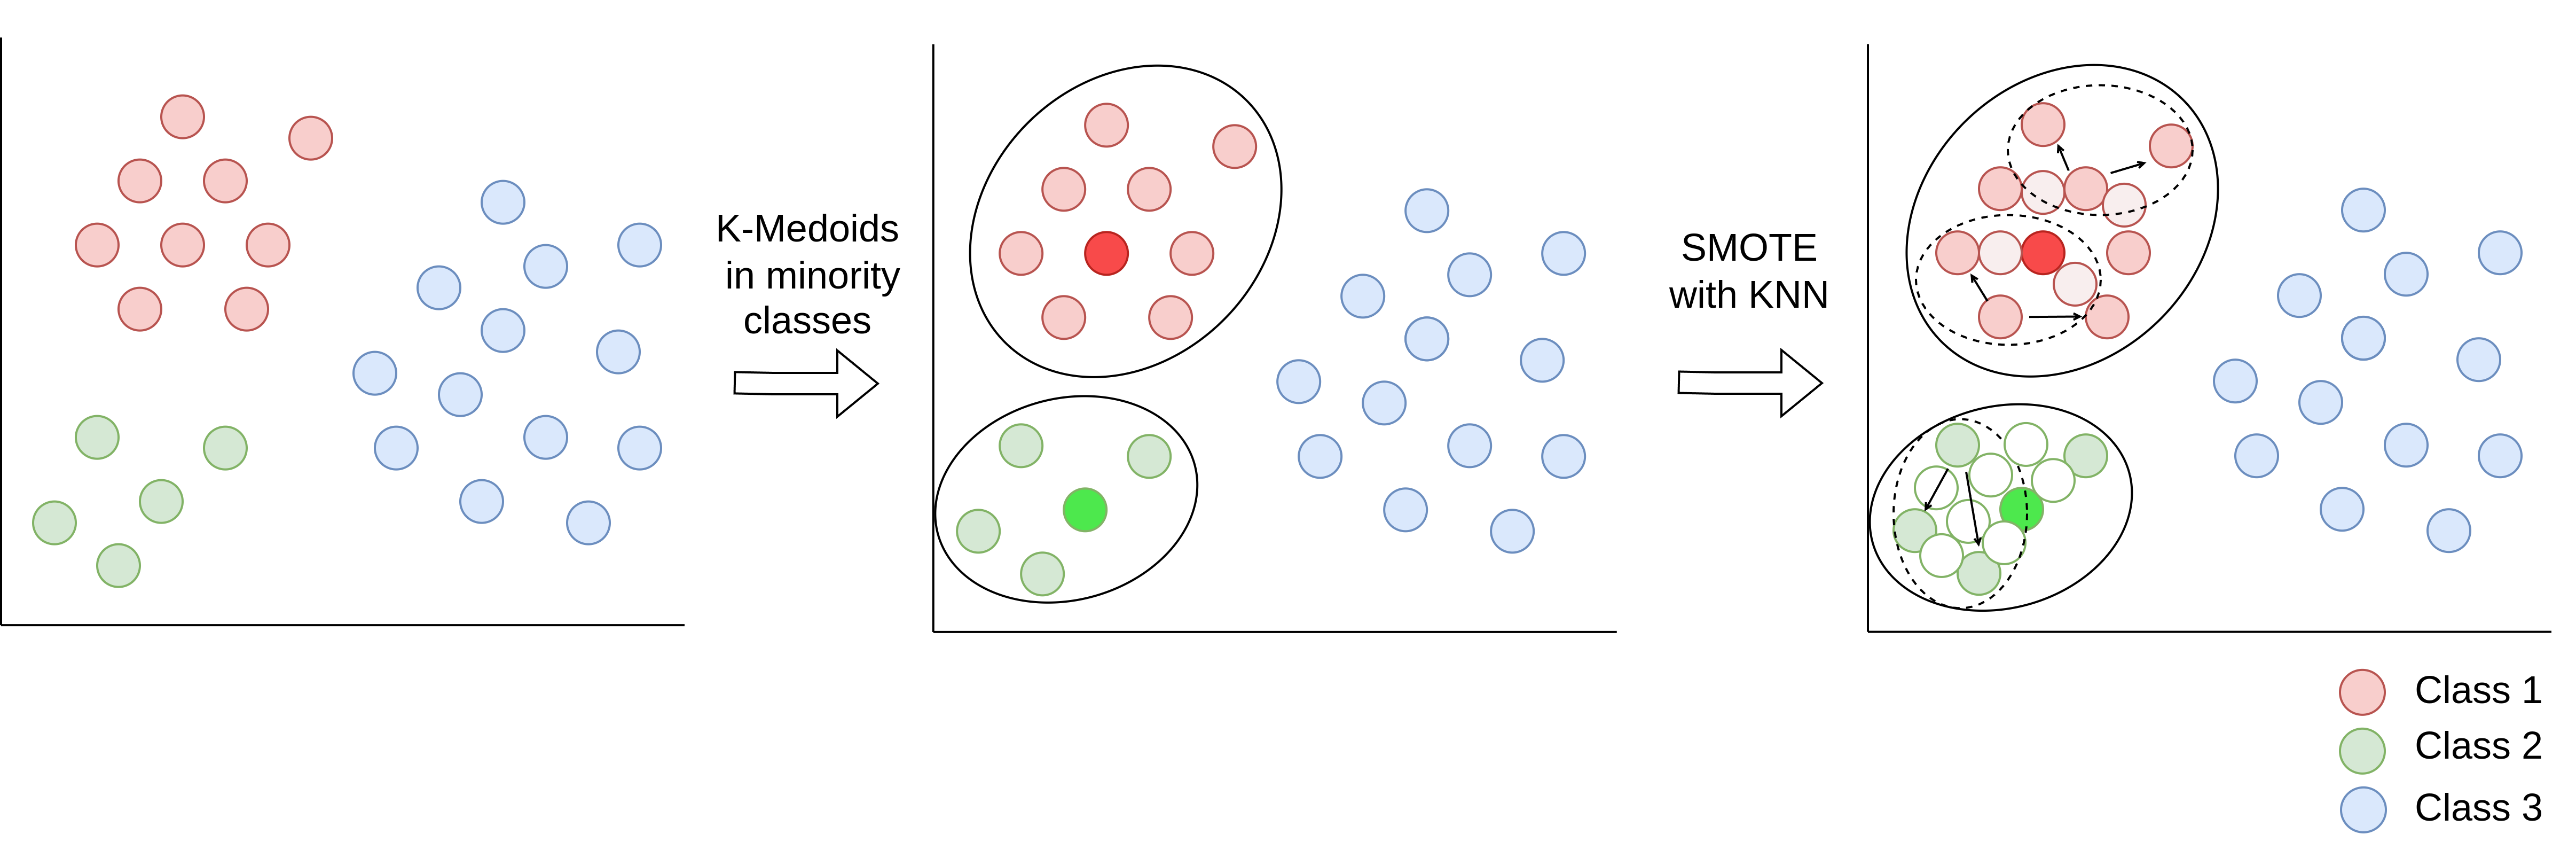
\includegraphics[width=1\linewidth]{figures/process.png}
    \caption{KM-SMOTE method working scheme.}
    \label{fig:Process_km_smote}  
\end{figure}





\begin{algorithm}[H]
    \caption{KM-SMOTE Algorithm}
    \label{Alg:K-medoidsSMOTE}
    \KwData{Features $X$, Labels $y$, Distance Metric $distance$, Number of Clusters $n\_clusters$}
    \vspace{0.1cm}
    \KwResult{$X\_resampled$, $y\_resampled$}
    \vspace{0.1cm}
    
    \textbf{Resampling Process:}\\
    Initialize $X\_resampled \leftarrow X$, $y\_resampled \leftarrow y$ \\

    classes $\leftarrow$ All classes but majority class \\ 
    
    \ForEach{class in $classes$}{
        $K-medoids$ $\leftarrow$ K-medoids($n\_clusters$, $distance$) \\
        Train $K-medoids$ on $X$[$class$] \\ %$K-medoids$.fit($X$[$class$])
        $clusters \leftarrow$ Assign data points in $X$[$class$] to clusters \\
        \ForEach{$cluster$ in $clusters$}{
            N $\leftarrow \frac{\text{samples in the majority class} - \text{samples in current class}}{\text{number of clusters}}$

            Initialize and train $NearestNeighbors$ with $distance$ on cluster's samples \\
            %Initialize NearestNeighbors with $distance$ \\
            %Train NearestNeighbors on cluster's samples \\
            %neighbors  \leftarrow NearestNeighbors($distance$) of cluster's samples \\

            \ForEach{$i \leftarrow 1$ to N}{
                $s_1$ $\leftarrow$ Select random sample from $cluster$ \\
                $neighbors$ $\leftarrow$ Get nearest neighbors of $s_1$ using $NearestNeighbors$ \\
                $s_2$ $\leftarrow$ Select random sample from $neighbors$ \\
                %Select two random samples: $s_1$, $s_2$ \\

                $synthetic\_sample$ $\leftarrow$ $s_1$ + rand(0,1) $\cdot$ ($s_2-s_1$) \\
                $X\_resampled \leftarrow X\_resampled \cup synthetic\_sample$
                $y\_resampled \leftarrow y\_resampled \cup class$
            }
        }
    }
    \KwRet{$X\_resampled$, $y\_resampled$}\\
\end{algorithm}


\section{Experiments} \label{sec:experimental}


\subsection{Methodology}
We follow the pipeline shown in Figure \ref{fig:pipeline}. Data is collected from various sources: License Plate Recognition (LPR), the General Directorate of Traffic (DGT), the National Institute of Statistics (INE), and survey questionnaires. Initially, these data are analyzed and preprocessed, which includes cleaning, handling missing values, and normalization. This allows us to build a dataset focused on our smart village area. Once this step is completed, we extract relevant features to build a model. We then conduct an evaluation process that involves using different classification models, oversampling methods, and distance metrics on the models. We use the models K-Nearest Neighbors (KNN), Logistic Regression (LR), Support Vector Machine (SVM), and Multilayer Perceptron (MLP). The oversampling methods we use are SMOTE, K-means-SMOTE, and CURE-SMOTE. The distances we use are Euclidean (associated with the $L_2$ norm) and Manhattan (associated with the $L_1$ norm). We use these results to build a model in which the new predicted variable, ``likelihood'', is used to enrich the dataset for the dynamic pricing algorithm. 

In the second phase, with that predicted likelihood, we build a dynamic pricing algorithm, in which the previous model will contribute with that behavioral component to the price assignment. Finally, to measure the impact of the different features in that dynamic pricing algorithm, we build a regression model.
\begin{figure}[H]
    \centering
    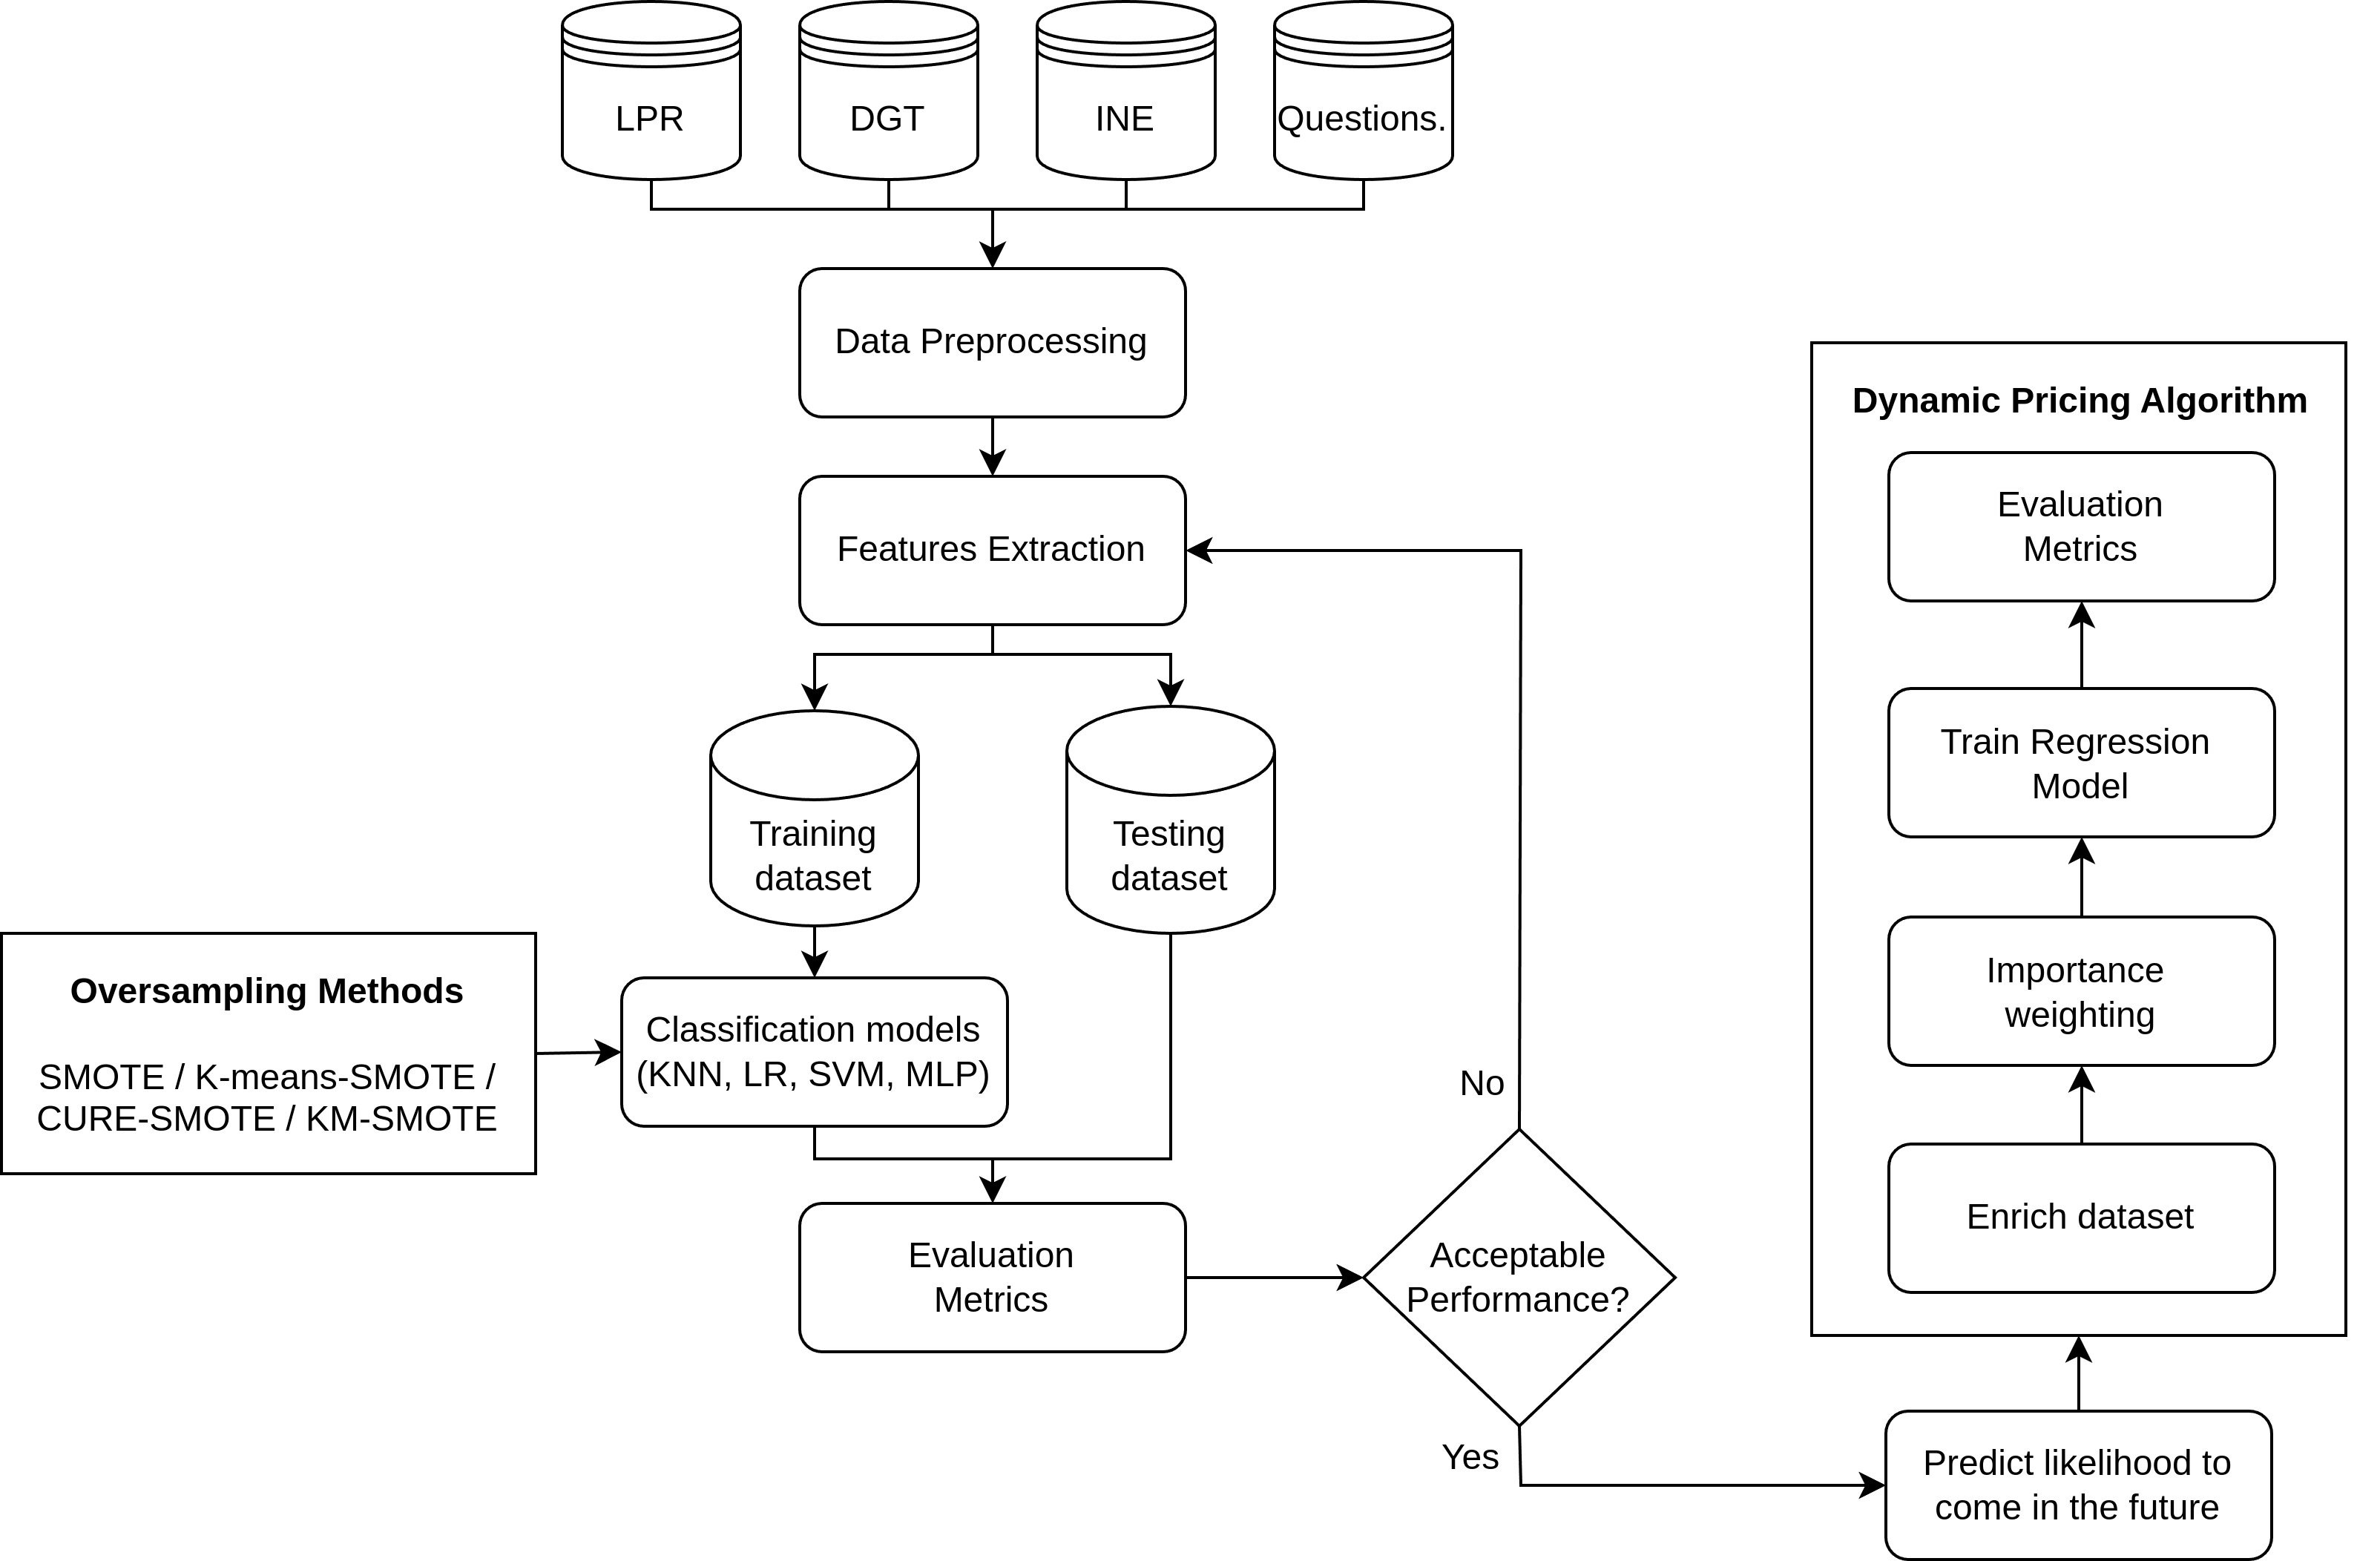
\includegraphics[width=1\linewidth]{figures/pipeline.png}
    \caption{Pipeline schema}
    \label{fig:pipeline}
\end{figure}


\subsection{Data overview} \label{sec:data_overview}

\begin{comment}
To test the algorithm, we studied the predisposition of tourists to return in the future if a parking fee is implemented in the areas of Pampaneira, Capileira, and Bubion, three villages in the Alpujarra, near the Sierra Nevada National Park in Granada, Spain. This intention was gathered from questionnaire data, which was complemented with data from a sensor network in the area. This system consists of four Hikvision LPR IP cameras with Deep Learning-based Automatic Number Plate Recognition (ANPR). These cameras are strategically located to detect the entrance and exit of the villages, allowing the movements within the villages to be easily tracked. This dataset consists of approximately 226,000 instances, collected from February 2022 to July 2023. Additionally, we used web scraping to obtain the environmental label of each vehicle from its license plate. Finally, we complemented this dataset with data from the Spanish Directorate-General for Traffic (DGT), resulting in a combined dataset that includes behavioral information, vacation information, and geographical data of each vehicle that enters the area. This information can be summarized as follows:

\begin{itemize}
    \item \textbf{Tourist behavior}: Consists of spatio-temporal information for each tourist in the area. Variables in this set include kilometers traveled in the area (calculable from the sequence of appearances in the different cameras), number of entries, number of nights of the stay, whether they would be willing to return in the future if a parking fee is imposed (class label), etc.
    \item \textbf{Vacation information}: Contains variables such as whether the entry was in high or low season, entry on holidays or not, entry on a workday or weekend, etc.
    \item \textbf{Vehicle information}: Variables such as CO2 emissions, environmental label (B, C, Eco, or Blue), place of origin, and number of seats of the vehicle belong to this category.
\end{itemize}
\end{comment}


To test the different algorithms in our smart village area, we build a dataset from various sources including LPR, DGT, INE, and questionnaires, where instances are joined with the vehicle's license plate number. The dataset is available in \citep{duran_lopez_2024} and it comprises:
\begin{enumerate}
    \item \textbf{Visitation data} collected from a sensor network consisting of four Hikvision LPR IP cameras equipped with Deep Learning-based License Plate Recognition (LPR) technology.
    \item \textbf{Geographic data} sourced from the Spanish Directorate-General for Traffic (DGT\footnote{\url{https://sede.dgt.gob.es/es/vehiculos/}}), providing variables related to vehicle origin.
    \item \textbf{Demographic data} sourced from the National Statistics Institute (Spanish: Instituto Nacional de Estadística, INE\footnote{\url{https://www.ine.es/index.htm}}), offering further insights into vehicle origins.
    \item \textbf{Questionnaire} responses gathered in January, March, and July 2023, excluding local residents to maintain proportional representation similar to the LPR data. Questionnaires, which were conducted in a parking lot, included questions such as license plate number, residential postcode, total visits to the area, overnight stays, etc. One question assessed respondents' inclination to revisit the area if a parking toll is implemented, with response options: ``visit more'', ``visit less'', or ``no affect''. This variable serves as the prediction class for this dataset.
\end{enumerate}


All this information has been preprocessed and analyzed, including normalization of variables, imputation of missing values, and elimination of outliers, so that the information is ready for the proposed algorithm. A summary of the main characteristics of the dataset can be seen in the table \ref{tab:summary}.


\begin{table}[H] 
\centering
\resizebox{\textwidth}{!}{%
\begin{tabular}{cccc}
\hline
\textbf{Data Category} & \textbf{Variable} & \textbf{Data Type} & \textbf{Description} \\ \hline
\multirow{7}{*}{\begin{tabular}[c]{@{}c@{}}Vehicle Behavior\\ (LPR Cameras)\end{tabular}} 
 & visit\_time & Time & Total duration of stay. \\
 & distance & Float & Total distance covered in kilometers within the area. \\
 & nights & Integer & Count of nights stayed. \\
 & visits\_dif\_weeks & Integer & Number of different weeks with at least one visit. \\
 & visits\_dif\_months & Integer & Number of different months with at least one visit. \\
 & fidelity & Float & Visits after maintaining a fidelity of at least five days. \\
 & cumulative\_entries & Integer & Total count of entries. \\ \hline
 
\multirow{6}{*}{\begin{tabular}[c]{@{}c@{}}Holiday Context\end{tabular}} 
 & num\_holiday & Integer & Total number of holidays. \\
 & num\_workday & Integer & Total number of workdays. \\
 & num\_high\_season & Integer & Number of days spent during high season. \\
 & num\_low\_season & Integer & Number of days spent during low season. \\
 & entry\_in\_holiday & Boolean & Entry during holidays. \\
 & entry\_in\_high\_season & Boolean & Entry during high season. \\ \hline
 
\multirow{3}{*}{\begin{tabular}[c]{@{}c@{}}Demographic and\\ Economic Data\\ (INE)\end{tabular}} 
 & avg\_gross\_income & Float & Average gross income of the origin area of the vehicle. \\
 & population & Integer & Population size of the orithin of the vehicle city/town. \\
 & is\_resident & Boolean & Tourist is resident from Pampaneira, Capileira or Bubión. \\ \hline
 
\multirow{4}{*}{\begin{tabular}[c]{@{}c@{}}Geographic Data\\ (DGT)\end{tabular}} 
 & km\_to\_dest & Float & Distance in kilometers between the origin of the vehicle and destination. \\
 & num\_seats & Integer & Number of seats in the vehicle. \\
 & environmental\_distinctive & String & Blue - ECO - C Green - B Yellow (scraped). \\
 & co2\_emissions & Float & CO2 emissions in g/km (imputed). \\ \hline
 
Questionnaires 
 & likelihood & Integer & Predicted class label indicating the likelihood to repeat the visit. \\ \hline
\end{tabular}%
}
\caption{Selected Dataset Variables}
\label{tab:summary}
\end{table}






%Poner tabla resultados







%COMENTAR POR ALGÚN LADO CÓMO DE % ESTÁ NUESTRO DATASET



\subsection{Model Training}

We use a 5-fold cross-validation method to validate our models. This method divides the dataset into five equal parts. Each model is trained and tested five times, with each part used once as the test set and four times as part of the training set. This method helps us evaluate the model's performance and stability across different conditions. We divide the data in three sets, training, validation and test, with a 70-10-20 proportion, respectively. %The variable to predict, ``likelihood to come'' has three clases: ``No affect'', ``More'', ``Less''.

We avoid using accuracy as a metric in those imbalanced datasets because it tends to favor the majority class and might give a high score while overlooking the minority class. Instead, we use Recall, F1-Score, G-Mean to evaluate our classifiers across the dataset \citep{he2009learning,fawcett2006introduction}. These metrics ensure that our models are effective across all categories, not just the dominant class. 


\subsection{Results} \label{sec:results}


We use four different classifiers to evaluate the proposed algorithm and compared it across various algorithms: KNN, MLP, LR, and SVM. The Table \cref{tab:combined_results} shows the results of the differents metrics with the diffents algorithms we used: the base case (None), SMOTE, K-means-SMOTE, CURE-SMOTE and KM-SMOTE with $L_1$ and $L_2$ norm.


\begin{table}[H]
\caption{Performance comparison of oversampling techniques across classifiers}
\centering
\resizebox{\textwidth}{!}{%
\begin{tabular}{lccc|ccc|ccc|ccc}
\hline
\textbf{Method} & \multicolumn{3}{c}{\textbf{KNN}} & \multicolumn{3}{c}{\textbf{MLP}} & \multicolumn{3}{c}{\textbf{LR}} & \multicolumn{3}{c}{\textbf{SVM}} \\
 & Recall & F1-Score & G-Mean & Recall & F1-Score & G-Mean & Recall & F1-Score & G-Mean & Recall & F1-Score & G-Mean \\
\hline
None & 0.6408 & 0.6315 & 0.6972 & 0.6311 & 0.6326 & 0.6815 & 0.7212 & 0.6103 & 0.6728 & 0.5701 & 0.4497 & 0.5712 \\
SMOTE & 0.6117 & 0.6121 & 0.6830 & 0.7087 & 0.7046 & 0.7374 & 0.7401 & 0.6041 & 0.6842 & 0.5437 & 0.4236 & 0.5780 \\
k-means-SMOTE & 0.6311 & 0.6315 & 0.6901 & 0.6893 & 0.6895 & 0.7346 & 0.6214 & 0.6142 & 0.6748 & 0.5534 & 0.4447 & 0.5840 \\
CURE-SMOTE & 0.6408 & 0.6413 & 0.6981 & 0.6311 & 0.6324 & 0.6822 & 0.6214 & 0.6103 & 0.6728 & 0.5437 & 0.4236 & 0.5737 \\
KM-SMOTE+$L_1$ & \textbf{0.6712} & \textbf{0.6592} & \textbf{0.7133} & \textbf{0.7206} & \textbf{0.7064} & \textbf{0.7586} & \textbf{0.7622} & \textbf{0.6436} & \textbf{0.7139} & 0.6112 & \textbf{0.6001} & \textbf{0.6761} \\
KM-SMOTE+$L_2$ & 0.6563 & 0.6413 & 0.6981 & 0.7114 & 0.6908 & 0.7492 & 0.7412 & 0.6319 & 0.6987 & \textbf{0.6128} & 0.5962 & \textbf{0.6761} \\
\hline
\end{tabular}%
}
\label{tab:combined_results}
\end{table}




\begin{figure}[h]
    \centering
    \begin{minipage}{0.8\textwidth}
        \centering
        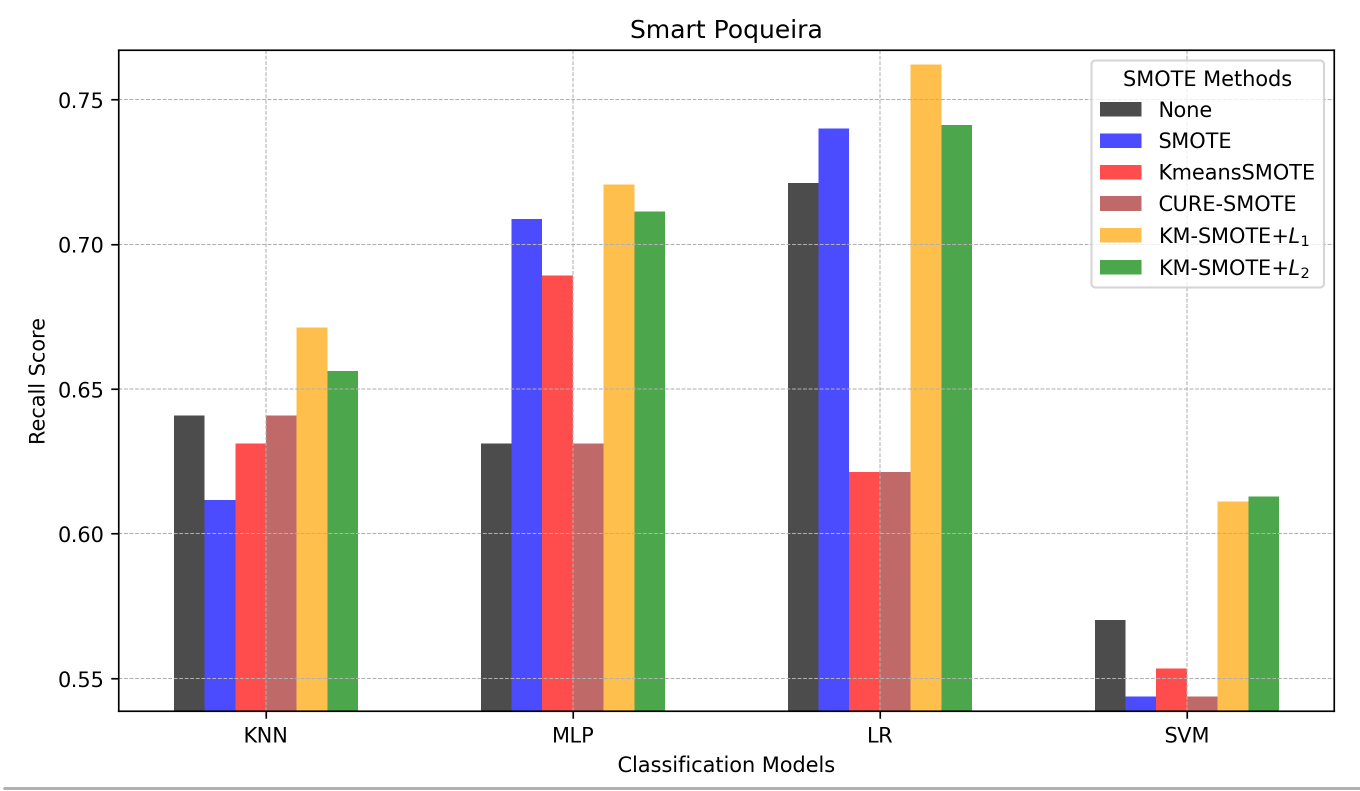
\includegraphics[width=\linewidth]{figures/recall.png}
        \caption{Recall comparison}
        \label{fig:grid_recall}
    \end{minipage}\\
    \begin{minipage}{0.8\textwidth}
        \centering
        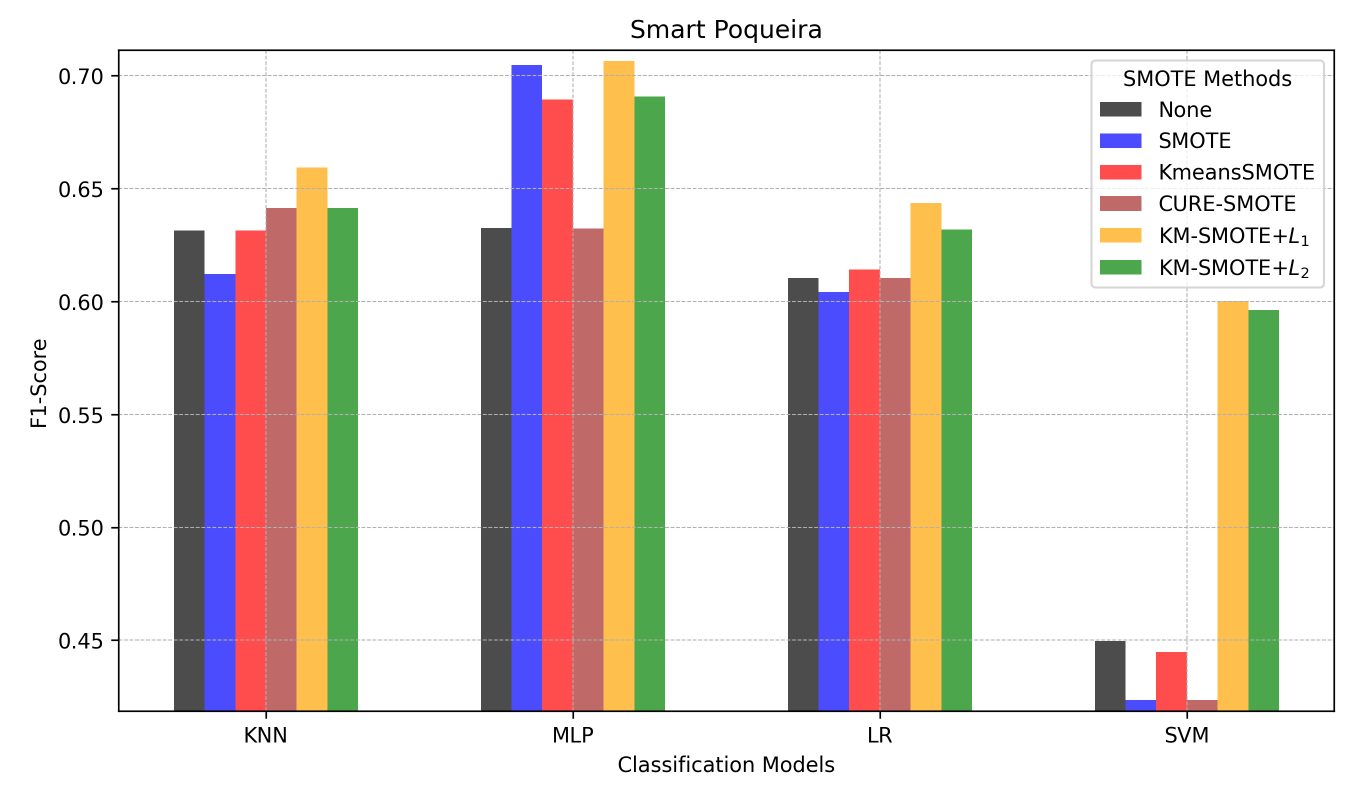
\includegraphics[width=\linewidth]{figures/f1score.png}
        \caption{F1-Score comparison across datasets}
        \label{fig:grid_f1}
    \end{minipage}\\
    \begin{minipage}{0.8\textwidth}
        \centering
        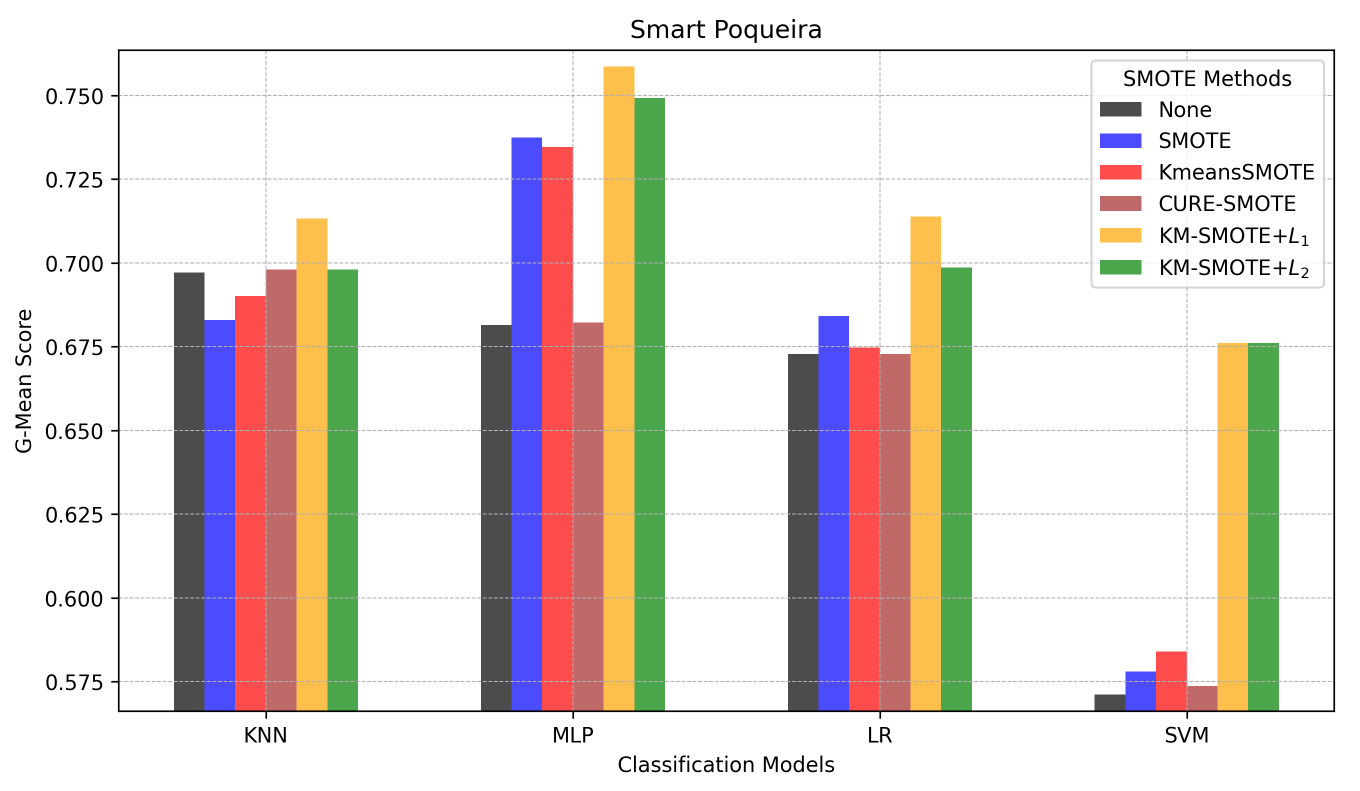
\includegraphics[width=\linewidth]{figures/gmean.png}
        \caption{G-Mean comparison across datasets}
        \label{fig:grid_gmean}
    \end{minipage}
\end{figure}






\subsection{Discussion} \label{sec:discussion}

There is noticeable variability in the results of the different classification algorithms used. KM-SMOTE achieves the best results in all metrics across all methods. As observed in Table \ref{tab:combined_results} and Figures \ref{fig:grid_recall}, \ref{fig:grid_f1}, and \ref{fig:grid_gmean}, KM-SMOTE in its both versions on SVM shows a significant improvement in the results compared to the other methods. In KNN, MLP, and LR, KM-SMOTE also improves performance, but the improvement is not as pronounced. The other clustering-based algorithms, K-means-SMOTE and CURE-SMOTE, do not perform as well. In fact, in the recall score shown in Figure \ref{fig:grid_recall}, the base case, SMOTE, without any previous clustering even yields better results.

KM-SMOTE with the $L_1$ norm, which utilizes the Manhattan distance, generally yields the highest scores across all classifiers. This significantly improves performance compared to the baseline and SMOTE, effectively balancing sensitivity and specificity across different classes, and managing noise and class imbalance more efficiently.









































\chapter{Dynamic Pricing Algorithm} \label{sec:dynamic}

%In the current business environment, price fixation is an important tool. Traditional models, such as fixed pricing, have been used in the past for their simplicity. However, these models have limitations in their ability to adapt to market fluctuations and user preferences, remaining unchanged regardless of varying conditions such as time, demand, or special events. Their limitation lies in their inability to adapt to changes in visitor behavior, potentially leading to inefficiencies in revenue generation and parking capacity management. These limitations have driven new approaches with dynamic pricing models. These models use real-time data on demand and user behavior, attempting to maximize profits without losing users. In contrast, a dynamic pricing algorithm offers a more flexible approach, adjusting parking fees based on a range of factors. This method allows prices to fluctuate in response to different conditions such as peak times, visitor influx, or special events. It is designed to optimize revenue generation by dynamically altering prices in line with current demand and other relevant variables.

%In our study of the Sierra Nevada National Park, we have a triple approach: environmental, economic, and social. To achieve this, we use data collected from 2022 to 2023 in the Alpujarra. In our approach, we will utilize the data collected from our cameras to either reward or penalize visits based on certain criteria. Moreover, the "Likelihood to Come in the Future" prediction, as discussed in the previous chapter, will play a key role in adjusting parking fees. By integrating this behavioral forecast, we aim to not only improve revenue but also better manage park attendance.

%Publicaciones relevantes:
%Dynamic Pricing in the Presence of Strategic Consumers (Besbes Zeevi, 2015)
%The Impact of Dynamic Pricing on Revenue Management (Talluri  Van Ryzin, 2006)
%Optimal Pricing Strategies for Seasonal Products (Phillips, 2005)


\section{Pricing Strategies}

We propose two pricing strategies to utilize on our data, which consists of various visit instances. Each instance in the dataset is represented by a vector of features. Table \ref{tab:data} shows the data representation.
\begin{table}[h]
  \centering
  \begin{tabular}{cccccc}
    \hline
    & \textbf{Feature 1} & \textbf{Feature 2} & \textbf{Feature 3} & $\ldots$ & \textbf{Feature m}  \\
    \hline
    Visit 1 & Value 1   & Value 2   & Value 3   & $\ldots$ & Value m   \\
    Visit 2 & Value 1   & Value 2   & Value 3   & $\ldots$ & Value m   \\
    $\vdots$ & $\vdots$ & $\vdots$  & $\vdots$  & $\ddots$ & $\vdots$  \\
    Visit n & Value 1   & Value 2   & Value 3   & $\ldots$ & Value m   \\
    \hline
  \end{tabular}
  \caption{Data Representation}
  \label{tab:data}
\end{table}


To determine the price of a tourist visit, the algorithm uses a rule-based method, where each feature contributes partially to the final price. The significance of variables varies, so the weights assigned to the features are not the same. To address this, we sort the features according to two different criteria.

\begin{enumerate}
    \item \textbf{Strategy 1}: We assign each variable an importance, and prices are determined accordingly. We order the variables in a descending sequence using a common ratio $r$, with $r \in (0,1)$. This implies that if the first variable has an importance $I$, the subsequent variable will have an importance of $r \cdot I$, and so on until the least important variable will have an assigned value of $r^{m-1} \cdot I$, where $m$ is the total number of features.
    
        \begin{table}[H]
        \centering
        \begin{tabular}{@{}cc@{}}
        \toprule
        \textbf{Feature} & \textbf{Importance} \\ \midrule
        $X_1$            & $I$                 \\
        $X_2$            & $r \cdot I$         \\
        $\vdots$         & $\vdots$            \\
        $X_m$            & $r^{m-1} \cdot I$   \\ \bottomrule
        \end{tabular}%
        \caption{Strategy 1}
        \label{strategyone}
        \end{table}
        
        This is done by employing a geometric progression of weights. The weight for the $k$-th feature is $w_k = r^{k-1}$, indicating the relative importance between consecutive features. We normalize the weights to ensure $\sum_{k=1}^{m} w_k = 1$. The normalization is as follows:
        \[
        \text{Normalized Importance}_k = \frac{r^{k-1} \cdot I}{I \sum_{j=0}^{m-1} r^j} = \frac{r^{k-1}}{\sum_{j=0}^{m-1} r^j}.
        \]

    
        This ensures that the sum of the normalized importances is 1, making them suitable for use as weights in the pricing algorithm.

    
    \item \textbf{Strategy 2}: We consider the existence of different categories within the set of all features, so the variables do not have a uniform descending order across the entire set. Instead, we assign different weights within each category, ordering the features within each category using Strategy 1. This strategy ensures that features are prioritized appropriately within their respective categories. We present this strategy as follows:


    \begin{table}[H]
    \centering
    \begin{tabular}{@{}ccc@{}}
    \toprule
    \textbf{Category}           & \textbf{Feature}   & \textbf{Importance}                                     \\ \midrule
    \multirow{3}{*}{Category 1} & $\text{Feature}_{1,1}$    & $I_{1,1}$                                                    \\
                                & $\vdots$           & $\vdots$                                                \\
                                & $\text{Feature}_{1,t_1}$ & $r_1^{t_1-1} \cdot I_{1,1}$ \\ \midrule
    \multirow{3}{*}{Category 2} & $\text{Feature}_{2,1}$    & $I_{2,1}$                                                    \\
                                & $\vdots$           & $\vdots$                                                \\
                                & $\text{Feature}_{2,t_2}$ & $r_2^{t_2-1} \cdot I_{2,1}$ \\ \midrule
    \multicolumn{3}{c}{$\vdots$}                                                                                    \\ \midrule
    \multirow{3}{*}{Category T} & $\text{Feature}_{T,1}$    & $I_{T,1}$                                                    \\
                                & $\vdots$           & $\vdots$                                                \\
                                & $\text{Feature}_{T,t_T}$ & $r_T^{t_T-1} \cdot I_{T,1}$ \\ \bottomrule
    \end{tabular}
    \caption{Strategy 2}
    \label{tab:strat_two}
    \end{table}

    
   If there are $T$ categories, denoted as $c_1, \ldots, c_T$, with associated weights $w_1, \ldots, w_T$, it holds that $w_1 + w_2 + \ldots + w_T = 1$. Additionally, within a category $c_i$, its assigned price $w_i$ satisfies:
    \[
    w_i = \sum_{j=0}^{t_i-1} r_i^j \cdot I_i, \quad i = 1, \ldots, T.
    \]
    
    Thus, it also holds that:
    \[
    \sum_{i=1}^{T} w_i = \sum_{i=1}^{T} \sum_{j=0}^{t_i-1} r_i^j \cdot I_i = 1.
    \]
\end{enumerate}


\subsection{Price Assignation}

The pricing function $P: \mathbf{X}_i \rightarrow \mathbb{R}$ assigns a price to each instance $i$ based on the weighted sum of its features. Here, $\mathbf{X}_i$ represents the feature vector for the $i$-th instance, and the function integrates weighted factors from different categories $c_1, \ldots, c_T$. The formula for the pricing function is:
\[
P(\mathbf{X}_i) = \alpha + (\beta - \alpha) \cdot \sum_{k=1}^{m} w_k \cdot f(x_{ik}, x_{\min k}, x_{\max k}),
\]

where:
\begin{itemize}
    \item $\alpha$ and $\beta$ are the predefined lower and upper bounds of the price, respectively.
    \item $w_k$, $k=1, \ldots, m$, are the weights derived from Strategy 1 or Strategy 2, with $\sum_{k=1}^{m} w_k = 1$.
    \item $f(x_{ik}, x_{\min k}, x_{\max k})$ is the Min-Max normalization function. To scale each feature $x_{ik}$ to the range $[0, 1]$, we apply a modified version of the Min-Max normalization function:
    \[
    f(x_{ik}, x_{\min k}, x_{\max k}) = \begin{cases}
        \frac{x_{ik} - x_{\min k}}{x_{\max k} - x_{\min k}}, & \text{if higher value of the feature is better}, \\
        1 - \frac{x_{ik} - x_{\min k}}{x_{\max k} - x_{\min k}}, & \text{if lower value of the feature is better}.
    \end{cases}
    \]
    \item $x_{ik}$ represents the value of the $k$-th feature for instance $i$, $x_{\min k}$ is the minimum value, and $x_{\max k}$ is the maximum value of the $k$-th feature across all instances.
\end{itemize}

In the price assignment process, we use the normalized and encoded feature values to compute the weighted average. The computed weighted average is then scaled between the predefined bounds $\alpha$ and $\beta$ to produce the final price. This systematic approach ensures that each feature's contribution is properly accounted for, resulting in a fair and accurate pricing mechanism based on the tourist's characteristics.




%For a new vehicle, its features are input into the model, and the model calculates a predicted price based on the learned coefficients. This prediction is a linear combination of the vehicle's features, each contributing to the final price in proportion to its coefficient in the model. Thus, the model provides a systematic and quantifiable approach to pricing, based on the characteristics of each vehicle.


\section{Experiments}

We consider the same dataset from Section \ref{sec:data_overview}, which is derived from the study by \cite{duran_lopez_2024}. In this section, we conclude with the final part of the pipeline shown in Figure \ref{fig:pipeline}. Here, we use the likelihood output feature obtained after applying different classification comparisons to our data as input. This behavioral variable contributes to the dynamic pricing algorithm for price assignment, along with the features listed in Table \ref{tab:used}.



\subsection{Data Preparation}

We create a new dataset containing only environmental, socio-economic, and behavioral variables to assign prices to each vehicle. The objective is that vehicles scoring better in these variables will have a lower price, while those scoring worse will have a higher price. Table \ref{tab:used} shows the variables we use in this study, along with the category to which they belong. The table also indicates whether a higher value of the feature is better.


\begin{table}[h]
\centering
\begin{tabular}{@{}cccc@{}}
\toprule
\textbf{Category}         & \textbf{Variable} & \textbf{Type} & \textbf{Better High} \\ \midrule
\multirow{3}{*}{Environmental} & co2\_emissions & Numeric & False \\
                              & distance & Numeric & False \\
                              & num\_seats & Numeric & True \\ \midrule
\multirow{5}{*}{Socio-economic} & entry\_in\_holiday & Categorical & False \\
                                & entry\_in\_high\_season & Categorical & False \\
                                & is\_resident & Categorical & True \\
                                & overnight & Categorical & True \\
                                & visit\_hours & Numeric & True \\ \midrule
\multirow{2}{*}{Behavioral} & cumulative\_entries & Numeric & True \\ 
                            & likelihood\_to\_come & Categorical & True \\ \bottomrule
\end{tabular}%
\caption{Description of variables with Better High column}
\label{tab:used}
\end{table}


For this analysis, we separate the variables into categorical and numeric types. We encode categorical variables as binary values (0 or 1) based on their specific conditions. For instance, ``is\_resident'' is 1 if the individual is a resident of Alpujarra and 0 otherwise. For numeric variables, we determine the lower and upper bounds using the Interquartile Range (IQR). The IQR is defined as $IQR = Q3 - Q1$. Using the IQR, we calculate the minimum and maximum values ($x_{\min}$ and $x_{\max}$) for each variable based on their respective first quartile ($Q1$) and third quartile ($Q3$) from historical data. The formula is as follows:
\[
[x_{\min}, x_{\max}] = [Q1 - 1.5 \cdot IQR, Q3 + 1.5 \cdot IQR].
\]

\begin{comment}
To scale each feature to the range $[0,1]$, we apply a modified version of the Min-Max normalization function to each feature, defined as $\mathbb{R}^3 \rightarrow [0,1]$:
\[
f(x, x_{\min}, x_{\max}) = \begin{cases}
    1 - \frac{x - x_{\min}}{x_{\max} - x_{\min}}, & \text{if not Better High}, \\
    \frac{x - x_{\min}}{x_{\max} - x_{\min}}, & \text{if Better High}.
\end{cases}
\]
\end{comment}

The ``Better High'' column from Table \ref{tab:used} indicates whether higher values are preferable. If this parameter is false, the normalized value is inverted to reflect that lower values are better \cite{witten2005practical}. This inversion is applied to both numerical and categorical variables to ensure they are appropriately scaled and encoded. This method ensures that values near the maximum incur the maximum cost, and values near the minimum incur the minimum cost for each variable, thus accurately reflecting their influence on the final price calculation.



\subsection{Regression Model}

We create a regression model to understand the impact of each feature on the final price. By analyzing the coefficients obtained from the regression model, we can determine how much each variable contribute to the final assigned price. This analysis allows us to assess the relative importance of different features with respect to the original assigned weights. Additionally, it helps to verify the effectiveness of our pricing algorithm by comparing the assigned weights in the price assignation with the learned coefficients from the regression model.

Given a new vehicle, we can test the predictive performance of our model using new data. Historical data was used to train the model, enabling us to identify any discrepancies or biases in the initial price assignment. The performance of the model is evaluated using the metrics MSE, MAE and $R^2$.


\subsection{Results}

We used Strategy 2 with the categories from Table \ref{tab:used}. The weights for the environmental, socio-economic, and behavioral categories were assigned equally $w_1 = w_2 = w_3 = \frac{1}{3}$. Within each category, we applied a common ratio of $r=0.9$. Additionally, we set the bounds $[\alpha, \beta] = [0.5, 1]$ to ensure that the prices fall within this range.

Table \ref{tab:results} shows the weights and the regression coefficients after applying Strategy 2. Table \ref{tab:metric_results} presents the results of the evaluation metrics. Figures \ref{fig:100samples} and \ref{fig:500samples} display the plots of the regression model with 100 and 500 samples, respectively.



\begin{table}[H]
\centering
\resizebox{\textwidth}{!}{%
\begin{tabular}{@{}ccccc@{}}
\toprule
\textbf{Category}         & \textbf{Feature} & \textbf{[Min, Max]} & \textbf{Weights} & \textbf{Regression coefficients} \\ \midrule
\multirow{3}{*}{Environmental} & co2\_emissions & [104.5, 140.5] & 0.1230 & 0.0146 \\
                              & distance & [0, 20.25] & 0.1107 & 0.0148 \\
                              & num\_seats & [2, 5] & 0.0996 & -1.4242e-06 \\ \midrule
\multirow{5}{*}{Socio-economic} & entry\_in\_holiday & N/A & 0.0814 & 0.0418 \\
                                & entry\_in\_high\_season & N/A & 0.0733 & 0.0393 \\
                                & is\_resident & N/A & 0.0659 & -0.0478 \\
                                & nights & [0, 7] & 0.0593 & -0.0192 \\
                                & visit\_hours & [0, 166.95] & 0.0534 & -0.0006 \\ \midrule
\multirow{2}{*}{Behavioral}  & likelihood\_to\_come & N/A & 0.1754 & -0.0240 \\
                            & cumulative\_entries & [0, 61] & 0.1579 & -0.0207 \\\bottomrule
\end{tabular}%
}
\caption{Results: Weights and regression coefficients}
\label{tab:results}
\end{table}







\begin{table}[h]
\centering
\begin{tabular}{cccc}
\hline
\textbf{Metric} & \textbf{MSE} & \textbf{MAE} & \textbf{R2} \\ \hline
Values          & 0.00064       & 0.0182 & 0.7933     \\ \hline
\end{tabular}%

\caption{Model Performance Metrics}
\label{tab:metric_results}
\end{table}


\newpage
\begin{figure}[H]
    \centering
    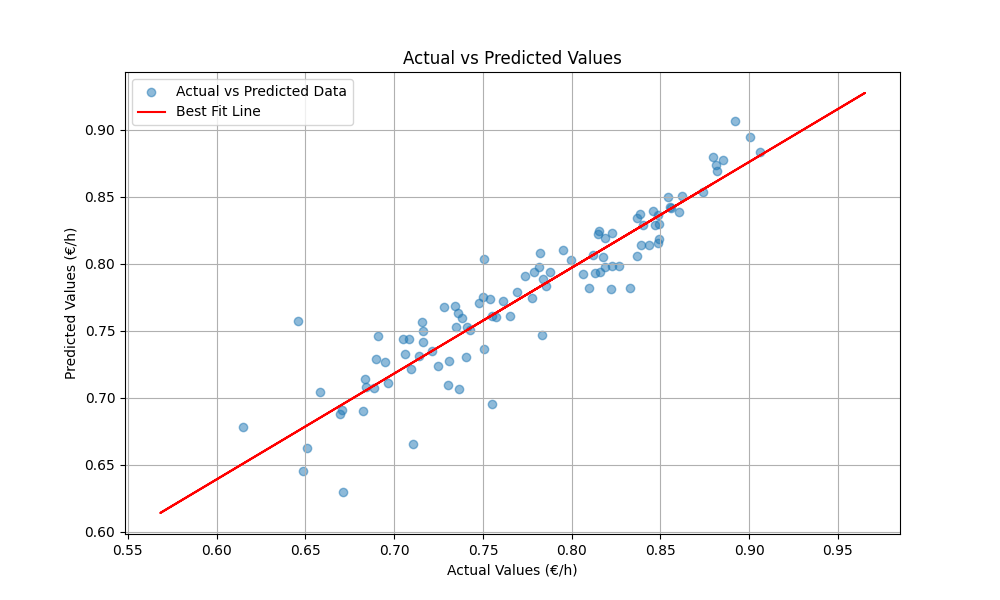
\includegraphics[width=0.8\textwidth]{figures/100.png}
    \caption{Regression model plot with 100 samples}
    \label{fig:100samples}
\end{figure}

\begin{figure}[H]
    \centering
    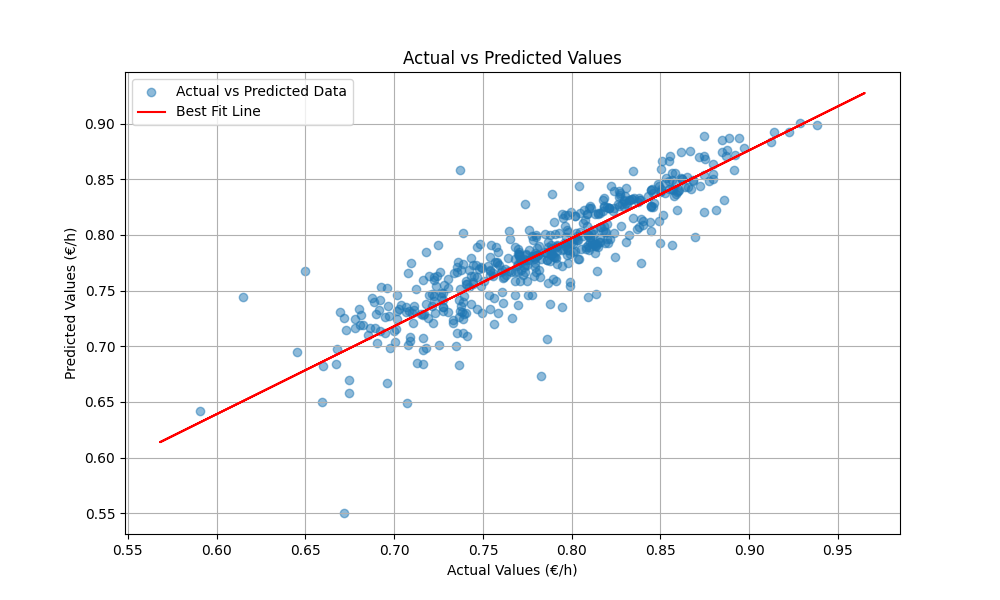
\includegraphics[width=0.8\textwidth]{figures/500.png}
    \caption{Regression model plot with 500 samples}
    \label{fig:500samples}
\end{figure}












\subsection{Discussion}

The weights from Table \ref{tab:results} align with the selected strategy, where the weights from each category $c_i$ sum to $w_i$, and the sum of all weights $w_1, \ldots, w_T$ equals 1. In this case, the features with the highest weights are the behavioral features likelihood\_to\_come and cumulative\_entries, which makes sense because there are only two features in their category.

According to the regression coefficients, positive values indicate that those features increase the price by that amount. Similarly, negative values indicate a decrease in the price. For example, for co2\_emissions, if a vehicle produces 104.5 g/km or lower (minimum bound), it will contribute 0 to the final price. Conversely, for 140.5 g/km or higher (maximum bound), it will contribute 0.0146 to the final price. Intermediate values will be assigned a contribution between 0 and 0.0146.




The MSE value of 0.00064 indicates a small average squared difference between the observed actual outcomes and the outcomes predicted by the model, suggesting high accuracy. The MAE value of 0.0182 further supports this, showing that the average magnitude of the errors in our predictions is low. The $R^2$ value of 0.7933 suggests that approximately 79.33\% of the variability in the price can be explained by the model, which is a good indication of the model's explanatory power. These results show that the pricing model is effective and reliable, with a strong predictive performance.


\chapter{Conclusions} \label{sec:conclusion}

This project is divided into two main parts. First, we introduced a novel oversampling method, KM-SMOTE, that combines K-medoids clustering with the SMOTE algorithm. It is specifically designed to enhance the performance of models on unbalanced datasets affected by noise and high dimensionality. We validated this method through a practical use case focused on smart villages, where we applied this algorithm to noisy sensor and survey data.

The proposed algorithm showed improvement in all metrics compared to other clustering-based algorithms and the original SMOTE. This improvement is due to the presence of outliers and noisy samples in this dataset, where the use of medoids contributes additional benefits. The class balancing proved effective in all cases, as indicated by the F1-Score, G-Mean, and Recall metrics. We also demonstrated that the problem of high dimensionality is reduced by using the Manhattan distance metric instead of the Euclidean metric. The results highlight the potential of this proposed algorithm, enabling data scientists and researchers to achieve more reliable and interpretable results, especially in scenarios with data imperfections.

Second, using the predictive power of our model, we predicted the willingness to return to the area after the implementation of a toll in a parking lot. Using that behavioral feature along with other environmental and socio-economic factors, we created a dynamic pricing algorithm to categorize vehicles based on these three dimensions: social, economic, and environmental, with a behavioral component. Each vehicle contributes according to these features. We used historical data to adjust variables in the model and created a dynamic price model using two strategies. Additionally, we developed a regression model to study how coefficients affect price weights, providing deeper insights into the pricing mechanism.

This contribution can be implemented in the Alpujarra region, assigning toll prices to vehicles. Accompanied by continuous data collection over several months, this dynamic pricing algorithm will allow dynamic price assignments to new vehicles entering the area. It will also prepare stakeholders to manage and prevent overcrowding in the Barranco de Poqueira, which was the main objective of this project.


\section{Limitations}

This study presents some limitations that open up opportunities for future research. Firstly, the amount of data collected is limited to specific periods and locations within the Sierra Nevada National Park, which may not be representative of all possible seasonal conditions or traffic variations. Additionally, the use of survey data may introduce biases due to subjective responses that the KM-SMOTE algorithm cannot fully learn. It may be beneficial to include other non-clustering-based and novel oversampling methods based on neural networks and compare them to assess KM-SMOTE's performance. Another limitation is that the data is collected from cameras, which sometimes suffer from outages, resulting in data loss. Finally, incorporating external factors beyond the specific set of features (environmental, socio-economic, and behavioral), such as public transportation policies or changes in road infrastructure, could provide a more comprehensive analysis. Although the KM-SMOTE algorithm has been shown to improve performance on our imbalanced and noisy dataset, future research should explore the integration of these additional factors to create a more comprehensive and adaptable pricing model. 

\section{Future Work}

The practical implementation of this model in the Alpujarra region will require continuous monitoring and adjustments based on real-time data to adapt to changing visitor dynamics and traffic patterns. Future work could focus on developing a real-time management platform that allows park managers to quickly and effectively adjust dynamic pricing policies, ensuring a sustainable balance between environmental preservation and tourism.

Additionally, future studies could investigate tourist patterns based on the routes they take within the national park. This could provide insights into the most visited areas and help in better managing foot traffic and preserving sensitive areas. Predicting tourism peaks using Google Trends is another avenue for future research, as it could help in anticipating high visitor periods and implementing proactive measures to manage the influx effectively.





\begin{comment}
\newpage
\appendix
\section*{Appendix - Dataset overview}
\label{ap:appendix}


We conducted a detailed analysis of the databases we will use in this section. As previously mentioned, we will work with two databases: the Surveys Database and the Visits Database.

\begin{itemize}
    \item The Surveys Database consists of a total of 539 instances, which collect information about the Natural Park. It contains variables that cannot be quantified using camera systems and measures the impact of the visit on tourists. Below, we present a grid of plot results:

    
    \begin{figure}[ht]
        \centering
        \begin{minipage}[b]{0.47\linewidth}
            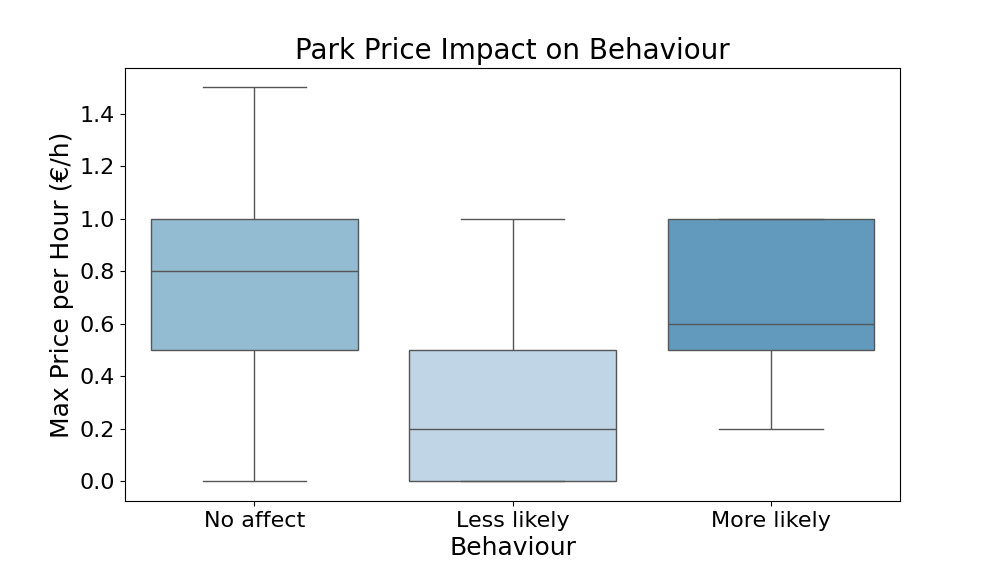
\includegraphics[width=\linewidth]{figures/first.png}
            \caption{Price Impact}
            \label{impact}
        \end{minipage}
        \hspace{0cm} % space between the images
        \begin{minipage}[b]{0.47\linewidth}
            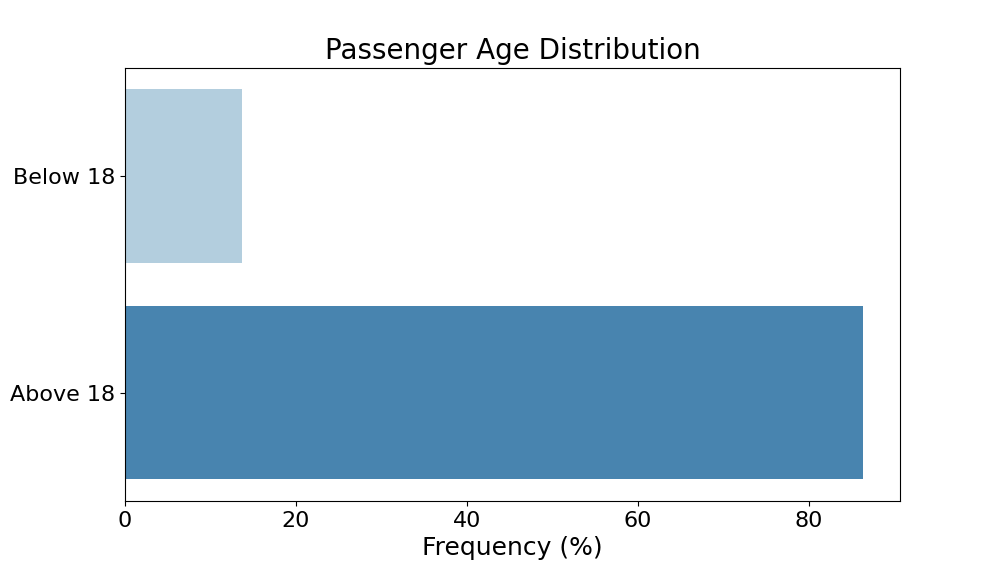
\includegraphics[width=\linewidth]{figures/third.png}
            \caption{Satisfaction}
            \label{satisfaction}
        \end{minipage}
    \end{figure}
    


    \begin{figure}[ht]
        \centering
        \begin{minipage}[b]{0.47\linewidth}
            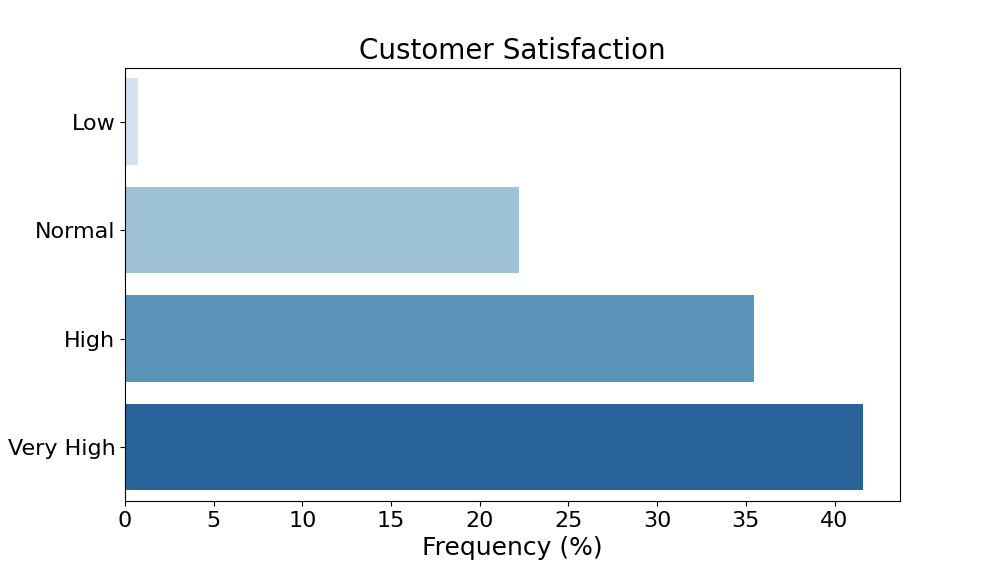
\includegraphics[width=\linewidth]{figures/second.png}
            \caption{Age Distribution}
            \label{distribution}
        \end{minipage}
        \hspace{0cm} % space between the images
        \begin{minipage}[b]{0.47\linewidth}
            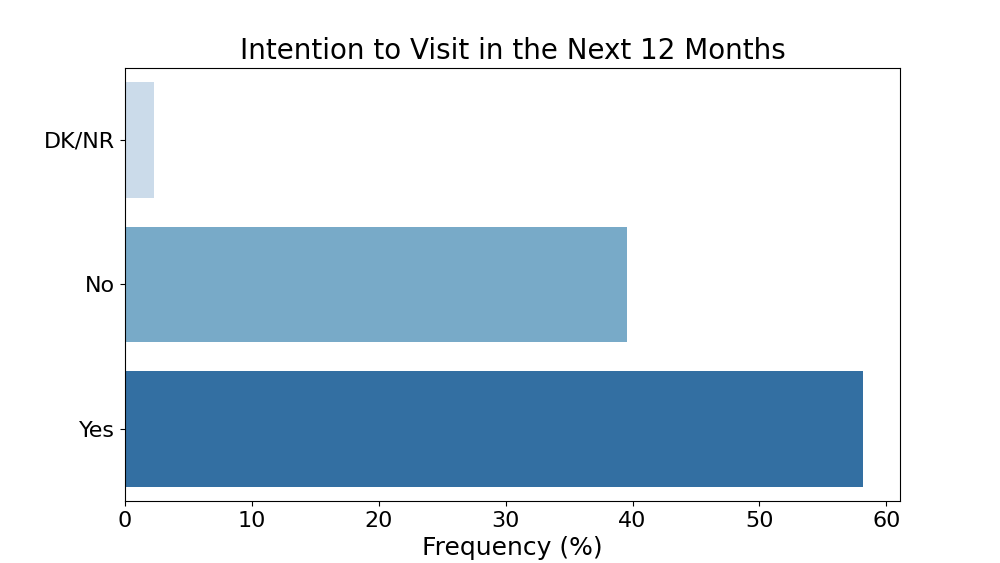
\includegraphics[width=\linewidth]{figures/fourth.png}
            \caption{Likelihood to come}
            \label{frequency}
        \end{minipage}
    \end{figure}



In the first graph \ref{impact}, we show how different customer groups relate to their willingness to pay for the implementation of this parking pricing system. Tourists can be grouped into three categories depending on their behaviour:

\begin{enumerate}
    \item \textbf{Less likely}: They are less inclined to visit in the future if a pricing system is implemented. The range of prices they are willing to pay is between 0€/h and 0.5€/h.
    \item \textbf{More likely}: This group, in favor of paying for parking, is willing to pay between 0.5€/h and 1€/h.
    \item \textbf{No effect}: They are indifferent to having to pay for parking. The range of prices they are willing to pay is between 0.5€/h and 1€/h.
\end{enumerate}

The second plot shows that over 80\% of tourists are older than 18 years old. Additionally, from the gathered data, we found that the median vehicle occupancy is around 53\%, meaning about 53\% of the seats in each vehicle are occupied. This information can be utilized to assess the environmental impact based on the number of seats in each vehicle.

Finally, the third and fourth graphs display tourist satisfaction and their intention to revisit within the next 12 months, respectively. These plots appear to be correlated, as the satisfaction levels of the tourists are either high or very high in more than 75\% of the cases, while only less than 25\% express normal or low satisfaction. This is reflected in the fact that 55\% of tourists want to repeat their trip and return in the next 12 months. This relationship can be effectively illustrated using the following heatmap:



\begin{figure}[H]
  \centering
  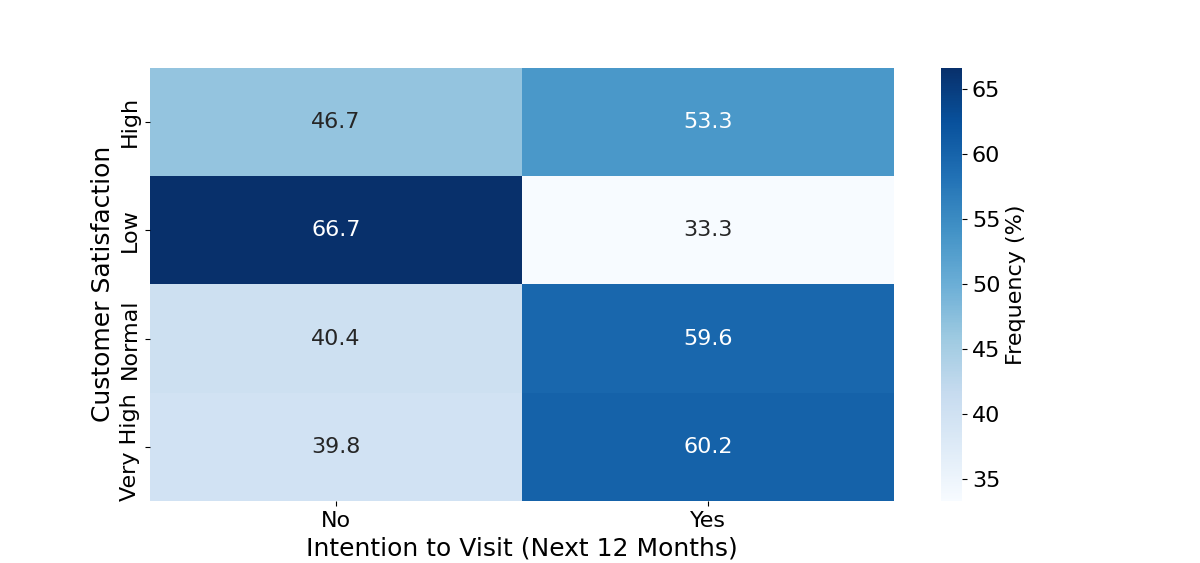
\includegraphics[width=0.9\textwidth]{figures/mix.png}
  \caption{Heatmap Satisfaction - Intention to visit}
  \label{heatmap}
\end{figure}

\newpage
\item On the other hand, the Visits Database contains around 226,000 entries of vehicles that have entered the zone, with a total of 45 features. The Visits Database can be divided into three parts:

    \begin{enumerate}
        \item \textbf{Vehicle Data}: This section describes characteristic information of each vehicle, such as the license plate number, which is the unique identifier. Other variables include the number of seats, CO2 emissions, and environmental distinctions. It is noteworthy that these variables have been obtained from the Dirección General de Tráfico (DGT).

        \item \textbf{Visit Data}: It contains information about each tourist's visit, such as entry and exit times, the route taken in the park, whether the visit occurred on a working day or holiday, among other details.

        \item \textbf{Residence Data}: This section includes variables like the neighborhood, city, province, autonomous community of origin, postal code, and number of inhabitants.
    \end{enumerate}
\end{itemize}

\end{comment}







%%%%%%%%%%%%%%%%%%%%%%% BIBLIOGRAFIA
%\printbibliography


\bibliographystyle{unsrt}
\bibliography{references.bib}
\end{document}